\documentclass[]{article}
\usepackage{lmodern}
\usepackage{amssymb,amsmath}
\usepackage{ifxetex,ifluatex}
\usepackage{fixltx2e} % provides \textsubscript
\ifnum 0\ifxetex 1\fi\ifluatex 1\fi=0 % if pdftex
  \usepackage[T1]{fontenc}
  \usepackage[utf8]{inputenc}
\else % if luatex or xelatex
  \ifxetex
    \usepackage{mathspec}
  \else
    \usepackage{fontspec}
  \fi
  \defaultfontfeatures{Ligatures=TeX,Scale=MatchLowercase}
\fi
% use upquote if available, for straight quotes in verbatim environments
\IfFileExists{upquote.sty}{\usepackage{upquote}}{}
% use microtype if available
\IfFileExists{microtype.sty}{%
\usepackage{microtype}
\UseMicrotypeSet[protrusion]{basicmath} % disable protrusion for tt fonts
}{}
\usepackage[margin=1in]{geometry}
\usepackage{hyperref}
\hypersetup{unicode=true,
            pdfborder={0 0 0},
            breaklinks=true}
\urlstyle{same}  % don't use monospace font for urls
\usepackage{longtable,booktabs}
\usepackage{graphicx,grffile}
\makeatletter
\def\maxwidth{\ifdim\Gin@nat@width>\linewidth\linewidth\else\Gin@nat@width\fi}
\def\maxheight{\ifdim\Gin@nat@height>\textheight\textheight\else\Gin@nat@height\fi}
\makeatother
% Scale images if necessary, so that they will not overflow the page
% margins by default, and it is still possible to overwrite the defaults
% using explicit options in \includegraphics[width, height, ...]{}
\setkeys{Gin}{width=\maxwidth,height=\maxheight,keepaspectratio}
\IfFileExists{parskip.sty}{%
\usepackage{parskip}
}{% else
\setlength{\parindent}{0pt}
\setlength{\parskip}{6pt plus 2pt minus 1pt}
}
\setlength{\emergencystretch}{3em}  % prevent overfull lines
\providecommand{\tightlist}{%
  \setlength{\itemsep}{0pt}\setlength{\parskip}{0pt}}
\setcounter{secnumdepth}{0}
% Redefines (sub)paragraphs to behave more like sections
\ifx\paragraph\undefined\else
\let\oldparagraph\paragraph
\renewcommand{\paragraph}[1]{\oldparagraph{#1}\mbox{}}
\fi
\ifx\subparagraph\undefined\else
\let\oldsubparagraph\subparagraph
\renewcommand{\subparagraph}[1]{\oldsubparagraph{#1}\mbox{}}
\fi

%%% Use protect on footnotes to avoid problems with footnotes in titles
\let\rmarkdownfootnote\footnote%
\def\footnote{\protect\rmarkdownfootnote}

%%% Change title format to be more compact
\usepackage{titling}

% Create subtitle command for use in maketitle
\providecommand{\subtitle}[1]{
  \posttitle{
    \begin{center}\large#1\end{center}
    }
}

\setlength{\droptitle}{-2em}

  \title{}
    \pretitle{\vspace{\droptitle}}
  \posttitle{}
    \author{}
    \preauthor{}\postauthor{}
    \date{}
    \predate{}\postdate{}
  

\begin{document}

\hypertarget{rooting-the-animal-tree-of-life}{%
\section{Rooting the animal tree of
life}\label{rooting-the-animal-tree-of-life}}

Yuanning Li\textsuperscript{1,3}, Xingxing Shen\textsuperscript{3},
Benjamin Evans\textsuperscript{2}, Antonis Rokas\textsuperscript{3}, and
Casey W. Dunn\textsuperscript{1}*

\textsuperscript{1}Department of Ecology and Evolutionary Biology, Yale
University

\textsuperscript{2}Yale Center for Research Computing, Yale University

\textsuperscript{3}Department of Biological Science, Vanderbilt
University

* Corresponding author,
\href{mailto:casey.dunn@yale.edu}{\nolinkurl{casey.dunn@yale.edu}}

\hypertarget{abstract}{%
\subsection{Abstract}\label{abstract}}

Phylogenomic studies based on hundreds to thousands of genes have
greatly improved our understanding of evolutionary relationships among
major animal lineages. However, a considerable debate still remains
regarding the animal origin, with Ctenophora-sister and Porifera-sister
emerging as the two primary hypotheses, comprising one of the most
difficult to resolve nodes in animal tree of life. Here, we
systematically explore the mechanisms that potentially cause the
incongruent results by synthesizing data and results from all previous
phylogenomic analyses, and perform new analyses with these data in a
consistent manner to characterize the differences between studies. We
find that gene sampling varies across studies, indicating that different
regions of the genomes are sampled with little overlap among data
matrices. More importantly, we find Porifera-sister can only be
recovered with more constraints, including using site-heterogeneous CAT
model and inclusive of the most closely related outgroups in several
matrices, whereas Ctenophora-sister is recovered in all other cases. We
next quantify the support of phylogenetic signal over the two hypotheses
and find substantial differences in the distribution of phylogenetic
signal between models and outgroup choice (especially CAT models). Last,
we show that recoding can be a problematic method for addressing
compositional variation in phylogenetic analyses. Our results provide a
comprehensive overview of the current understanding of the first
diverging animal branch and why different studies yield different
answers. Rather than embracing one hypothesis over another, we hope our
efforts provides an integrative overview of the challenge and provides
direction for future studies to address difficult phylogenetic problems.

\hypertarget{main}{%
\subsection{Main}\label{main}}

Phylogenomic analyses with genome-scale data have the potential to
revolutionize our understanding of the tree of life. However, over the
past decade, there has been considerable debate about the position of
the root of the animal phylogeny, with Ctenophora-sister (comb jelly)
and Porifera-sister (sponges) (Fig. 1) emerging as the two primary
hypotheses. Historically, there was little debate about the root of the
animal tree of life and Porifera-sister was widely accepted though
rarely tested. By contrast, there has long been uncertainty about the
relationship of Ctenophora to other animals\textsuperscript{1}. An
understanding of the first diverging animal lineage is critical for
scientists to reconstruct events that occurred early in animal
evolution, especially for the evolution of complex structures such as
cell types, nervous systems, and developmental patterns. However, a wide
consensus of animal origin has not been reached despite multiple
efforts.

The first phylogenomic study to include ctenophores\textsuperscript{2}
suggested a new hypothesis, now referred to as Ctenophora-sister, that
ctenophores are our most distant animal relative. Since then many more
studies have been published and extensive reanalyzed, some supporting
Ctenophora-sister, some Porifera-sister, and some neither (Table 1). It
has become clear that this is a very difficult phylogenetic challenge,
and as the problem has become better characterized, it has become an
interesting test-case to phylogenetic biologists beyond those concerned
with this particular biological problem. Work has been hindered, though,
because it has been difficult to directly compare results across studies
and synthesize findings to understand the broader patterns of support.
Here we synthesize data and results from all previous phylogenomic
analyses that tested Ctenophora-sister and Porifera-sister, and
reanalyze these data using standardized methods, and perform new
analyses to characterize differences between studies. We hope that this
effort provides an integrative overview of the challenge and provides
direction for future studies. We also hope that the work we have
conducted here, including consolidating all the datasets in one place
with consistent formats and species names, will enhance the technical
value of this interesting question to methods-focused investigators that
look to develop methods to address difficult phylogenetic problems.

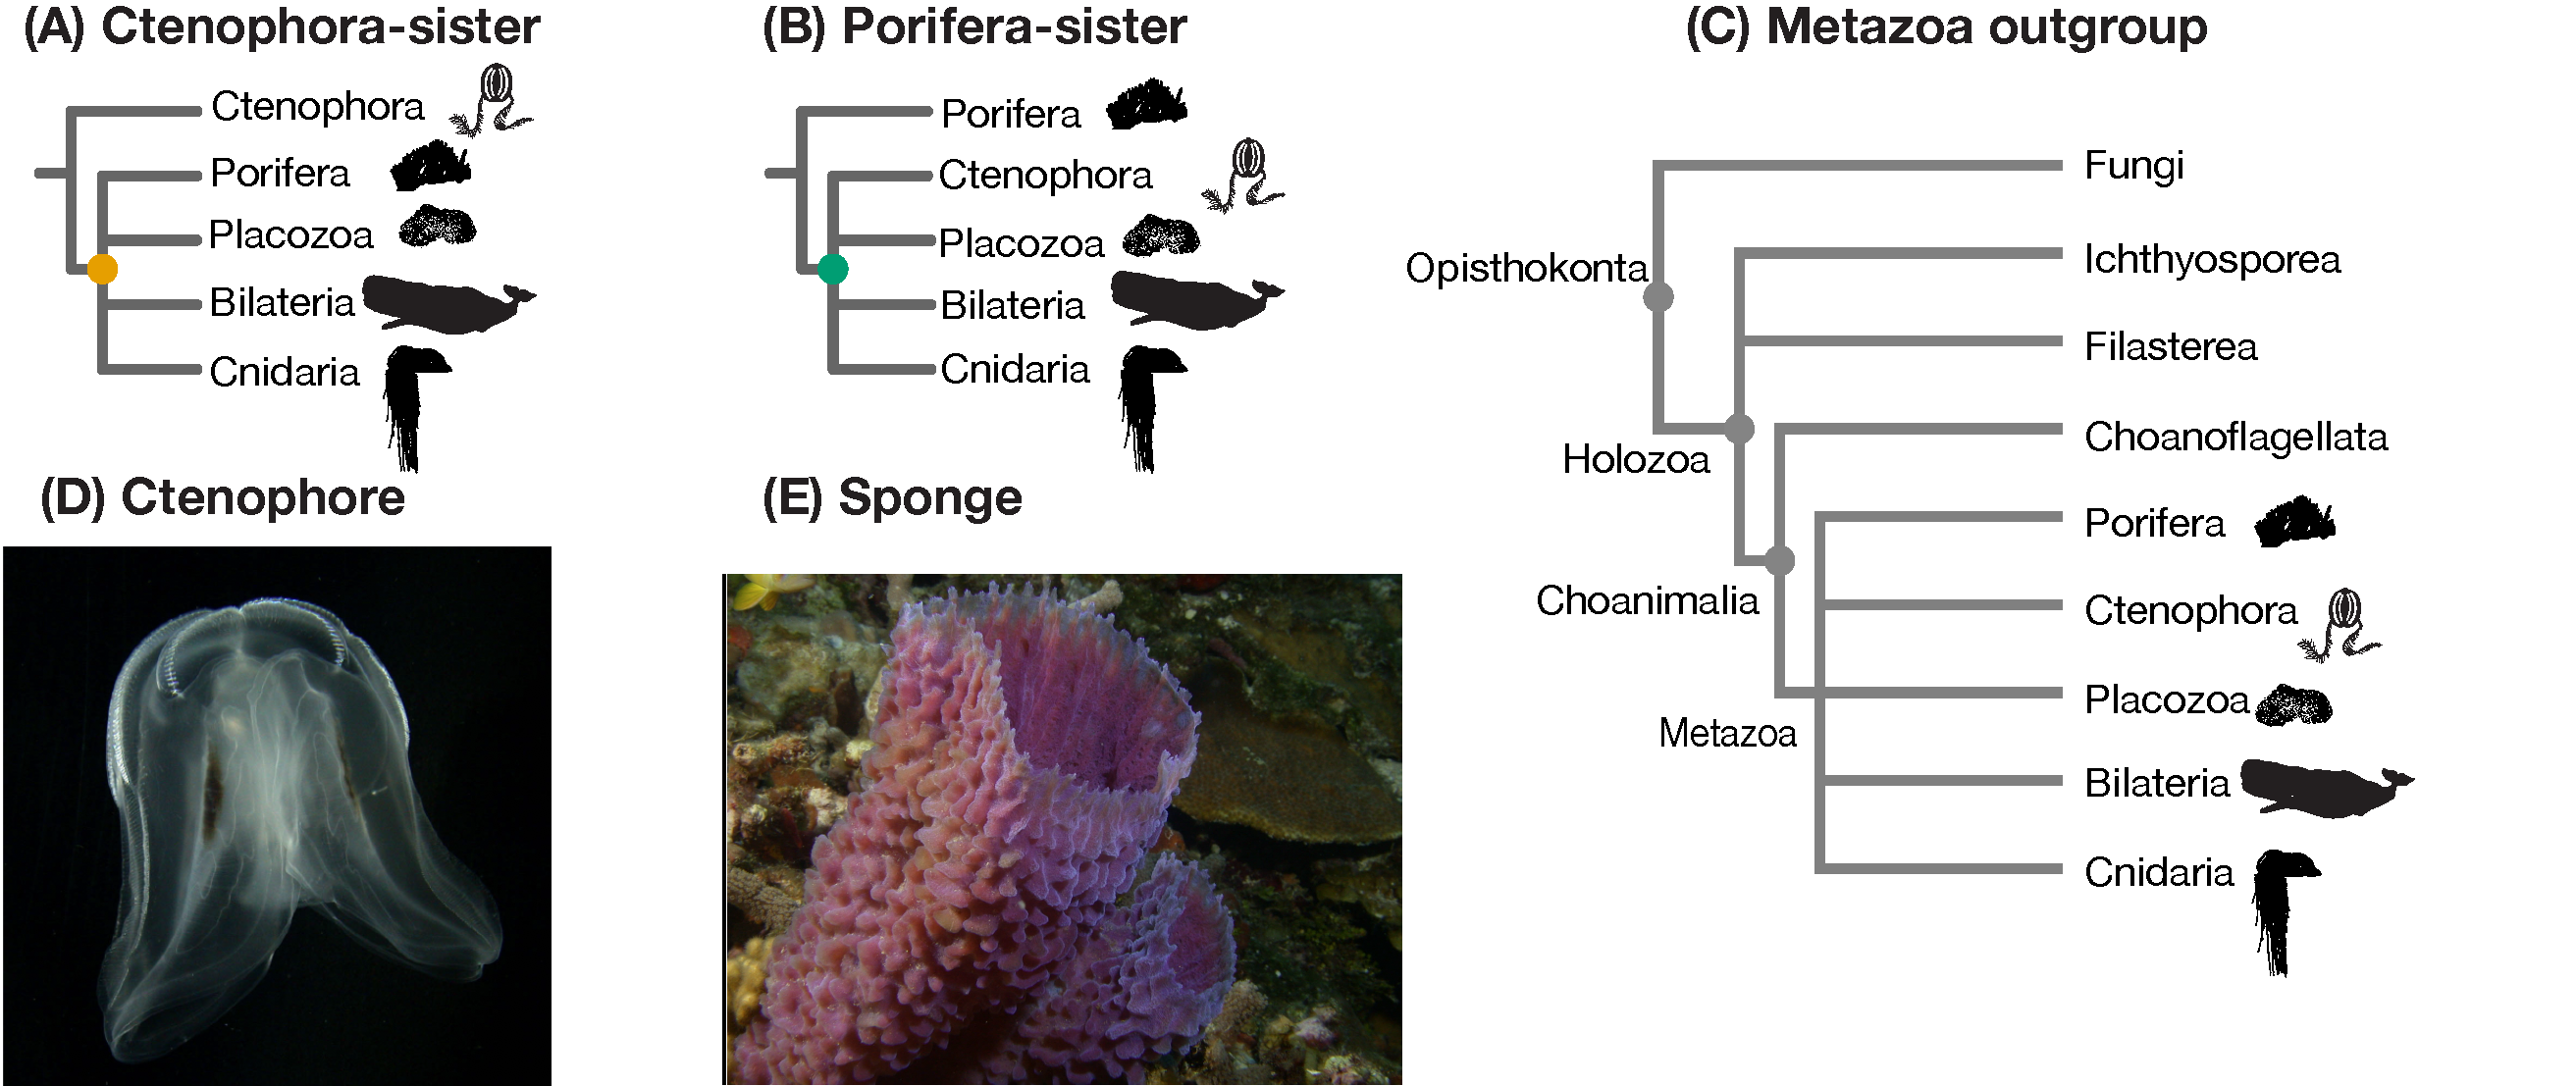
\includegraphics{figures/Figure_overview.png} \textbf{Fig. 1.} (A) The
Ctenophora-sister hypothesis posits that there is a clade (designated by
the orange node) that includes all animals except Ctenophora, and that
Ctenophora is sister to this clade. (B) The Porifera-sister hypothesis
posits that there is a clade (designated by the green node) that
includes all animals except Porifera, and that Porifera is sister to
this clade. Testing these hypotheses requires evaluating the support for
each of these alternative nodes. (C) The animals and their outgroup
choice, showing the three progressively more inclusive clades
Choanimalia, Holozoa, and Opisthokonta (designated by the blue node).
(D) A ctenophore. (E) A sponge.

\hypertarget{variation-across-studies}{%
\subsection{Variation across studies}\label{variation-across-studies}}

\hypertarget{models-of-molecular-evolution}{%
\subsubsection{Models of molecular
evolution}\label{models-of-molecular-evolution}}

Models of molecular evolution have several components that each consider
different aspects of the evolutionary process. The models that have been
used to model protein evolution in studies of the deep phylogeny have
largely differed according to three components: the exchangeability
matrix \(E\), the rate of evolution, and the state equilibrium
frequencies \(\Pi\). A detailed description of each component is in
Supplementary Results. Briefly, (1) the exchangeability matrix \(E\)
describes the rate at which one amino acid changes to another.
Exchangeability matrices have been used in the studies under
consideration here include: Poisson (or F81), WAG, LG, GTR, as they have
been used regularly in phylogenomic analyses; (2) While the
exchangeability matrix describes the relative rate of different changes
between amino acids, the actual rate can be further scaled, such as site
homogeneous rates and Gamma-rate heterogeneity; (3) the vector of
equilibrium frequencies \(\Pi\) describes the stationary frequency of
amino acids, such as empirical site-homogeneous, estimated
site-homogeneous, CAT site-heterogeneous\textsuperscript{3}, and C10-C60
models (C models).

Models can be assembled by selecting different options for all these
different components. The models that are applied in practice area
heavily influenced by engineering and computational costs, as well as
convention. For example, on the questions considered here, Poisson and
GTR exchangeability matrices have only been used in combination with CAT
site-heterogeneous models of equilibrium frequency. LG and WAG
exchangeability matrices have only been used with site homogeneous
estimates of equilibrium frequency. This is further confused by the
abbreviations that are used for models. Papers often discuss CAT and WAG
models as if they are exclusive, but these particular terms apply to
non-exclusive model components-- CAT refers to variation across sites
and WAG a particular exchangeability matrix. CAT is generally shorthand
for Poisson+CAT and WAG is shorthand for WAG+homogeneous equilibrium
frequency estimation. One could, though, run a WAG+CAT model, although
the computation time is much longer than Poisson+CAT model. To avoid
confusion on this point, we always specify the exchangeability matrix
first, followed by modifiers that describe the accommodation of
heterogeneity in equilibrium frequencies (\emph{e.g.}, CAT). If there
are no modifiers, then it is implied that site homogeneous models are
used. Moreover, the Gamma-rate heterogeinity is used in almost every
analysis.

\hypertarget{gene-sampling}{%
\subsubsection{Gene sampling}\label{gene-sampling}}

High-throughput sequencing is leading to exciting new data matrices for
phylogenomic analyses, potentially including hundreds or thousands of
genes to explore the root of animal phylogeny (Table 1). Although the
number of sampled genes might be different across studies, it is
reasonable to expect that a core set of orthologs should be present and
conserved across most animal genomes (\emph{e.g.}, animal BUSCO
genes\textsuperscript{4}). Surprisingly, gene composition and matrix
overlap has been rarely assessed across studies and most studies relied
on their own bioinformatic pipeline for determination of orthologs (for
details see Supplementary Results).

\hypertarget{outgroup-and-ingroup-taxon-sampling}{%
\subsubsection{Outgroup and ingroup taxon
sampling}\label{outgroup-and-ingroup-taxon-sampling}}

Outgroup selection (the taxa used to root the ingroup taxa) can
potentially affect the phylogenetic inference of animal evolution (Fig.
1C). Several studies have progressively removed more distantly related
outgroup taxa to test the effect of outgroup selection to ingroup
topology\textsuperscript{5,6}. Three progressively more inclusive clades
have often been investigated, including Choanomalia (Metazoa plus most
closely related Choanoflagellata), Holoza (Choanimalia plus more
distantly related holozoans) and Opisthokonta (Holozoa + Fungi). It has
been suggested the inclusion of more distant related (e.g.~Fungi)
outgroup taxa tend to recover Ctenophora-sister, whereas increasing
support of Porifera-sister often recovered when more closely related
outgroup taxa were used with site-heterogeneous CAT
models\textsuperscript{6}. In contrast of outgroup selection,
sensitivity to ingroup sampling has received less attention than
outgroup sampling. This may be because results have tended to be more
sensitive to outgroup sampling.

\hypertarget{data-recoding}{%
\subsubsection{Data-recoding}\label{data-recoding}}

Compositional heterogeneity (lineage-specific differences in amino acid
frequencies) was long thought has a major effect in resolving the animal
tree of life, especially for the deep animal
phylogeny\textsuperscript{7}. Variation in evolutionary rates across
taxa can lead to compositional heterogeneity that may lead to long
branch attraction of sponges or ctenophores\textsuperscript{8}. Feuda
\emph{et al}.\textsuperscript{9} has proposed to use data-recoding
method to reduce compositional heterogeneity in matrices. By discarding
information on which specific amino acid is found at each site in each
species and instead focusing on which groups those amino acids belong
to, they sought to reduce the impact of differences between species in
which particular amino acids within those groups are most frequent. By
reanalyzing Chang et al.~2015\textsuperscript{10} and Whelan et
al.~2015\textsuperscript{11}, they report that posterior predictive
analyses indicate recoded analyses have better model adequacy than
non-recoding analyses, and that Porifera-sister was strongly favored
under all recoding strategies using GTR-CAT models\textsuperscript{9}.
However, how the recoding methods impact phylogenetic inference has not
been well explored. Moreover, a recent simulation study has suggested
that non-recoding approaches significantly outperformed recoding
strategies\textsuperscript{12}. Thus, it is important to reevalute the
performance of the impact of data-recoding compared to non-recoding
methods in animal phylogeny.

\hypertarget{overview-of-published-analyses}{%
\subsection{Overview of published
analyses}\label{overview-of-published-analyses}}

Here, we synthesize data and results from all previous phylogenomic
analyses that tested Ctenophora-sister and Porifera-sister, including 17
data matrices from 12 studies (Table 1).

\begin{longtable}[]{@{}lllrrrlll@{}}
\caption{Table 1. Overview of data matrices used in this
study}\tabularnewline
\toprule
Study & Matrix & Clade & Number of gene partitions & Number of sites &
Number of taxa & Infered sister lineage & Journal &
Citations\tabularnewline
\midrule
\endfirsthead
\toprule
Study & Matrix & Clade & Number of gene partitions & Number of sites &
Number of taxa & Infered sister lineage & Journal &
Citations\tabularnewline
\midrule
\endhead
Dunn2008 & Dunn2008 & Opisthokonta & 150 & 21152 & 64 &
Ctenophora-sister & Nature & NA\tabularnewline
Philippe2009 & Philippe2009 & Opisthokonta & 129 & 30257 & 55 &
Porifera-sister & Current Biology & NA\tabularnewline
Hejnol2009 & Hejnol2009 & Opisthokonta & 1487 & 270580 & 94 &
Ctenophora-sister & Proc. Biol. Sci. & NA\tabularnewline
NA & Hejnol2009\_subsampled & Opisthokonta & 844 & 55594 & 94 &
Ctenophora-sister & NA & NA\tabularnewline
Nosenko2013 & Nosenko2013\_nonribo\_9187 & Opisthokonta & 35 & 9187 & 63
& Ctenophora-sister & Molecular Phylogenetics and Evolution &
NA\tabularnewline
Nosenko2013 & Nosenko2013\_ribo\_14615 & Opisthokonta & 87 & 14615 & 71
& Porifera-sister & NA & NA\tabularnewline
Ryan2013 & Ryan2013\_est & Opisthokonta & 406 & 88384 & 61 &
Ctenophora-sister & Science & NA\tabularnewline
Moroz2014 & Moroz2014\_3d & Opisthokonta & 114 & 22772 & 46 &
Ctenophora-sister & Nature & NA\tabularnewline
Whelan2015 & Whelan2015\_D1 & Opisthokonta & 251 & 59733 & 76 &
Ctenophora-sister & PNAS & NA\tabularnewline
Whelan2015 & Whelan2015\_D10 & Opisthokonta & 210 & 59733 & 70 &
Ctenophora-sister & NA & NA\tabularnewline
Whelan2015 & Whelan2015\_D20 & Opisthokonta & 178 & 81008 & 65 &
Ctenophora-sister & NA & NA\tabularnewline
Borowiec2015 & Borowiec2015\_Best108 & Choaimalia & 108 & 41808 & 36 &
Ctenophora-sister & BMC Genomics & NA\tabularnewline
Borowiec2015 & Borowiec2015\_Total1080 & Choaimalia & 1080 & 384981 & 36
& Ctenophora-sister & NA & NA\tabularnewline
Pisani2015 & Ryan2013\_est & Opisthokonta & 406 & 88384 & 60 &
Porifera-sister & PNAS & NA\tabularnewline
NA & Whelan\_D6 & Opisthokonta & 115 & 33403 & 70 & Porifera-sister & NA
& NA\tabularnewline
Chang2015 & Chang2015 & Opisthokonta & 170 & 51940 & 77 &
Ctenophora-sister & PNAS & NA\tabularnewline
Simion2017 & Simion2017 & Opisthokonta & 1719 & 401632 & 97 &
Porifera-sister & Current Biology & NA\tabularnewline
NA & Simion2017\_subsampled & Opisthokonta & 1719 & 110602 & 97 &
Porifera-sister & NA & NA\tabularnewline
Feuda2017 & Chang2015 & Opisthokonta & 170 & 51940 & 77 &
Ctenophora-sister & Current Biology & NA\tabularnewline
NA & WhelanD20 & Opisthokonta & 178 & 81008 & 65 & Porifera-sister & NA
& NA\tabularnewline
Whelan2017 & Whelan2017b\_full & Holozoa & 212 & 68062 & 80 &
Ctenophora-sister & Nature Ecology and Evolution & NA\tabularnewline
Whelan2017 & Whelan2017b\_strict & Choaimalia & 59 & 49388 & 76 &
Ctenophora-sister & NA & NA\tabularnewline
\bottomrule
\end{longtable}

\hypertarget{results-and-discussion}{%
\subsection{Results and Discussion}\label{results-and-discussion}}

\hypertarget{matrix-taxon-composition}{%
\subsubsection{Matrix taxon
composition}\label{matrix-taxon-composition}}

Taxa sampling plays a critical role in phylogenetic inference,
especially for the taxa whose phylogenetic position is poorly
understood. However, several data matrices have relatively skewed taxon
sampling, with more than 50\% taxa sampled in bilaterians compared to
other major animal lineages (Extended Data Fig. 1). These skewed data
matrices include two studies constructed from ESTs
(Dunn2008\textsuperscript{2} and Hejnol2009\textsuperscript{13}) and one
study from whole-genome data (Borrowiec2015\textsuperscript{14}).
Importantly, several earlier studies only include less than five
ctenophore species (Extended Data Fig. 1). The rest data matrices have
relatively balanced taxon composition, although the total number of
sampled taxon varies a lot. In general, increasing taxon sampling is
broadly accepted to improve phylogenetic inference and aid in the
placement of the earliest diverging animal lineage. Thus, it should be
noted that Whelan2017\textsuperscript{15} (has the most Ctenophore taxa)
and Simion2017\textsuperscript{16} (contains the most taxon sampling)
have much broader taxon sampling than other matrices.

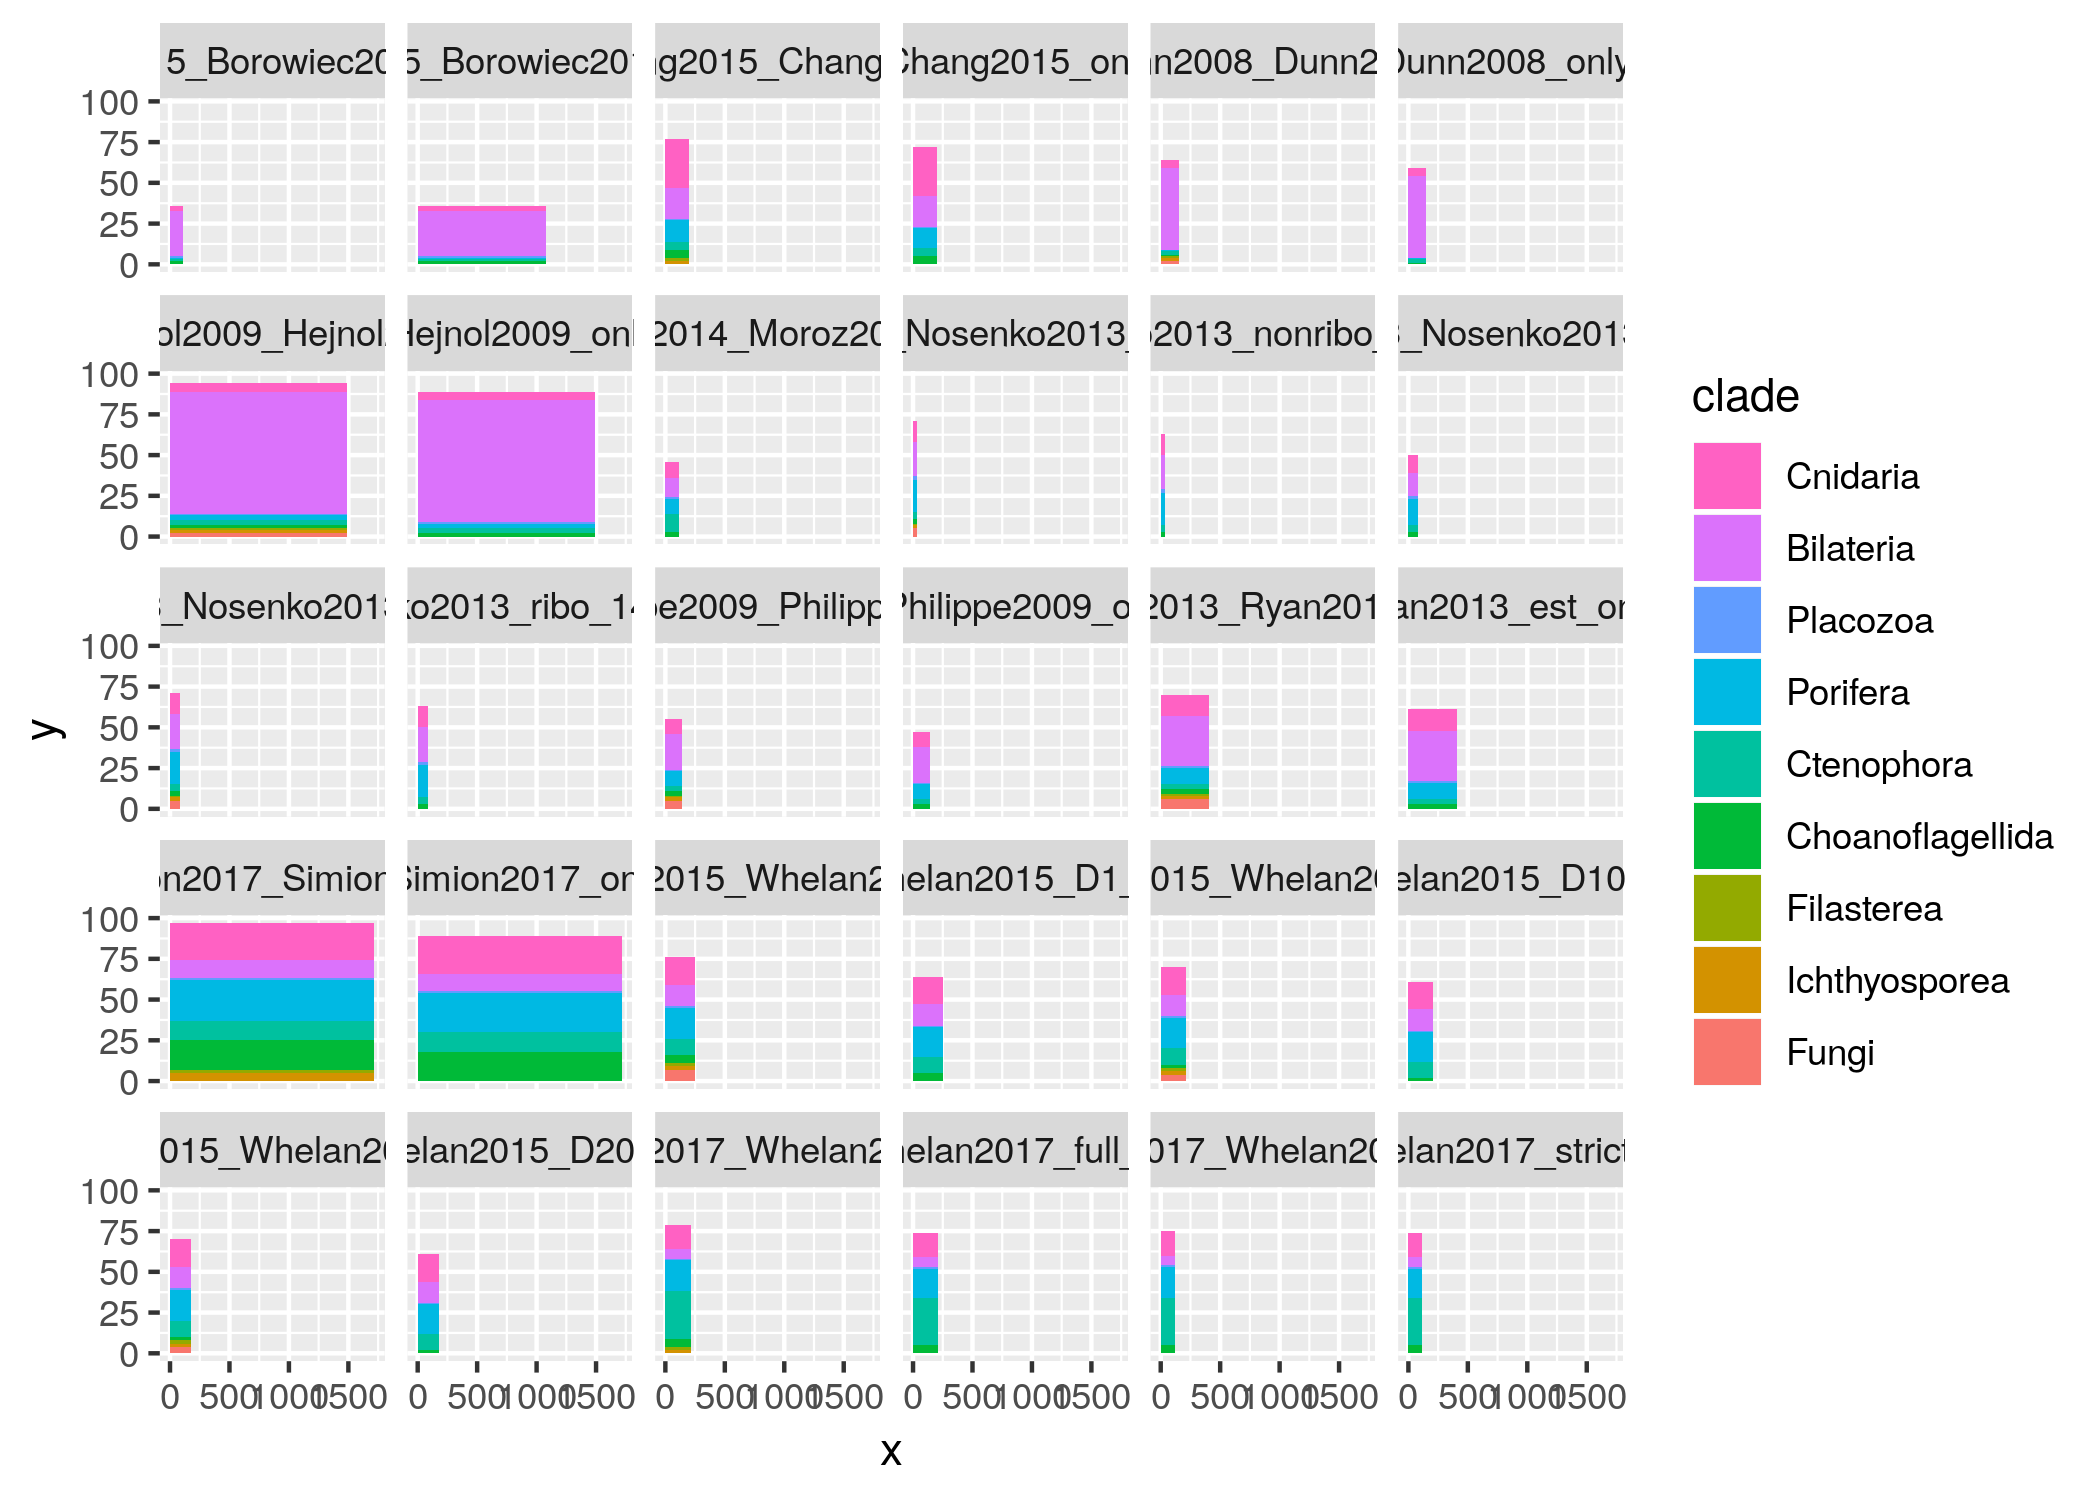
\includegraphics{manuscript_files/figure-latex/taxon_rectangles-1.pdf}

\textbf{Fig. Extended Data Fig. 1.} Each of the primary matrices
considered here, color coded by taxon sampling. Horizontal size is
proportional to the number of genes sampled, vertical size to the number
of taxa sampled.

\hypertarget{matrix-gene-composition-and-overlap}{%
\subsubsection{Matrix gene composition and
overlap}\label{matrix-gene-composition-and-overlap}}

Gene sampling also plays an essential role in phylogenomic analyses, and
most often rely on the concatenation of sampled genes for deep animal
phylogeny. It has been suggested that the concatenation assumes that
phylogenetic signal from genes that do not share the species phylogeny
will be overwhelmed by the signal from the majority of genes whose
genealogy mirrors that of the species evolutionary
history\textsuperscript{17}. However, large phylogenomic data matrices
potentially contain genes with conflicting or weak phylogenetic signal
that can lead to incongruence phylogenomic results, especially when
analyzing deeper node represents ancient divergence in the
tree\textsuperscript{18}. Thus, it is important to evaluate the gene
composition and matrix overlap to explore level of congruence of gene
sampling across different matrices.

We first used the Metazoa BUSCO genes\textsuperscript{{\textbf{???}}} to
evaluate gene composition from all data matrices and the result is
unexpected (Extended Data Fig. 2A). The animal BUSCO dataset contains
978 single-copy orthologs (identified from 64 animal taxa) that are most
likely shared by most animal genomes, and are commonly used to assess
the completeness of genome or transcriptomic
assemblies\textsuperscript{4}. The BUSCO genes also are frequently used
as markers in many large-scale phylogenomic studies (e.g.,
yeasts\textsuperscript{19}, spiders\textsuperscript{20}). Thus, it is
reasonable to expect that these conserved genes should present at a
higher percentage than non-BUSCO genes in most matrices. However, we
found that gene partitions from all matrices comprised less than 50\% of
BUSCO genes, even with several data matrices contain less than 20
percent (Extended Data Fig. 2B). Moreover, we identified number of
ribosomal RNA genes in each data matrix (Extended Data Fig. 2C). We
found Philippe2009, Nosenko2013\_ribo\_14615 and Chang2015 matrices
possessed much higher content of ribosomal genes than other matrices
(Extended Data Fig. 2D). We also annotated each gene partition against
SwissProt\textsuperscript{21} and Gene Ontology databases, and results
are shown in Supplementary Table 1.

Previous analyses have mainly focused on outgroup selection and/or model
fits in different data matrices, and the matrix overlap across different
studies has been rarely investigated since all these studies rely on
their own method for orthology inference. Our initial intent of
comparing matrix overlap across matrices was to construct a new matrix
with shared taxon and gene sampling to test specific hypotheses about
differences in support. The hypothesis is that although the
bioinformatics pipeline used for OG determination is different, most
larger data matrices should share a core set of orthologs. However, our
results show that surprisingly little overlap across all the data
matrices from different studies (Fig. 2). Thus, these results strongly
suggested that gene sampling largely varies across studies, indicating
that different regions of the genomes are sampled with little overlap
among different data matrices. Moreover, the little overlap among
studies may potentially lead to incongruent phylogenetic results and
difficult to directly compare results across studies.

\begin{verbatim}
## <ggproto object: Class CoordFixed, CoordCartesian, Coord, gg>
##     aspect: function
##     backtransform_range: function
##     clip: on
##     default: FALSE
##     distance: function
##     expand: TRUE
##     is_free: function
##     is_linear: function
##     labels: function
##     limits: list
##     modify_scales: function
##     range: function
##     ratio: 1
##     render_axis_h: function
##     render_axis_v: function
##     render_bg: function
##     render_fg: function
##     setup_data: function
##     setup_layout: function
##     setup_panel_params: function
##     setup_params: function
##     transform: function
##     super:  <ggproto object: Class CoordFixed, CoordCartesian, Coord, gg>
\end{verbatim}

\includegraphics{manuscript_files/figure-latex/gene_composition,-1.pdf}

\textbf{Extended Data Fig. 2.} Annotation and representation of BUSCO
and ribosomal genes in each data matrix. (A). The number of partitions
with BUSCO annotations in each matrix, relative to the number of
partitions. (B). The percentage BUSCO annotations in each matrix. (C).
The number of partitions with annotations of ribosomal genes in each
matrix, relative to the number of partitions. (D). The percentage
ribosomal genes in each matrix.

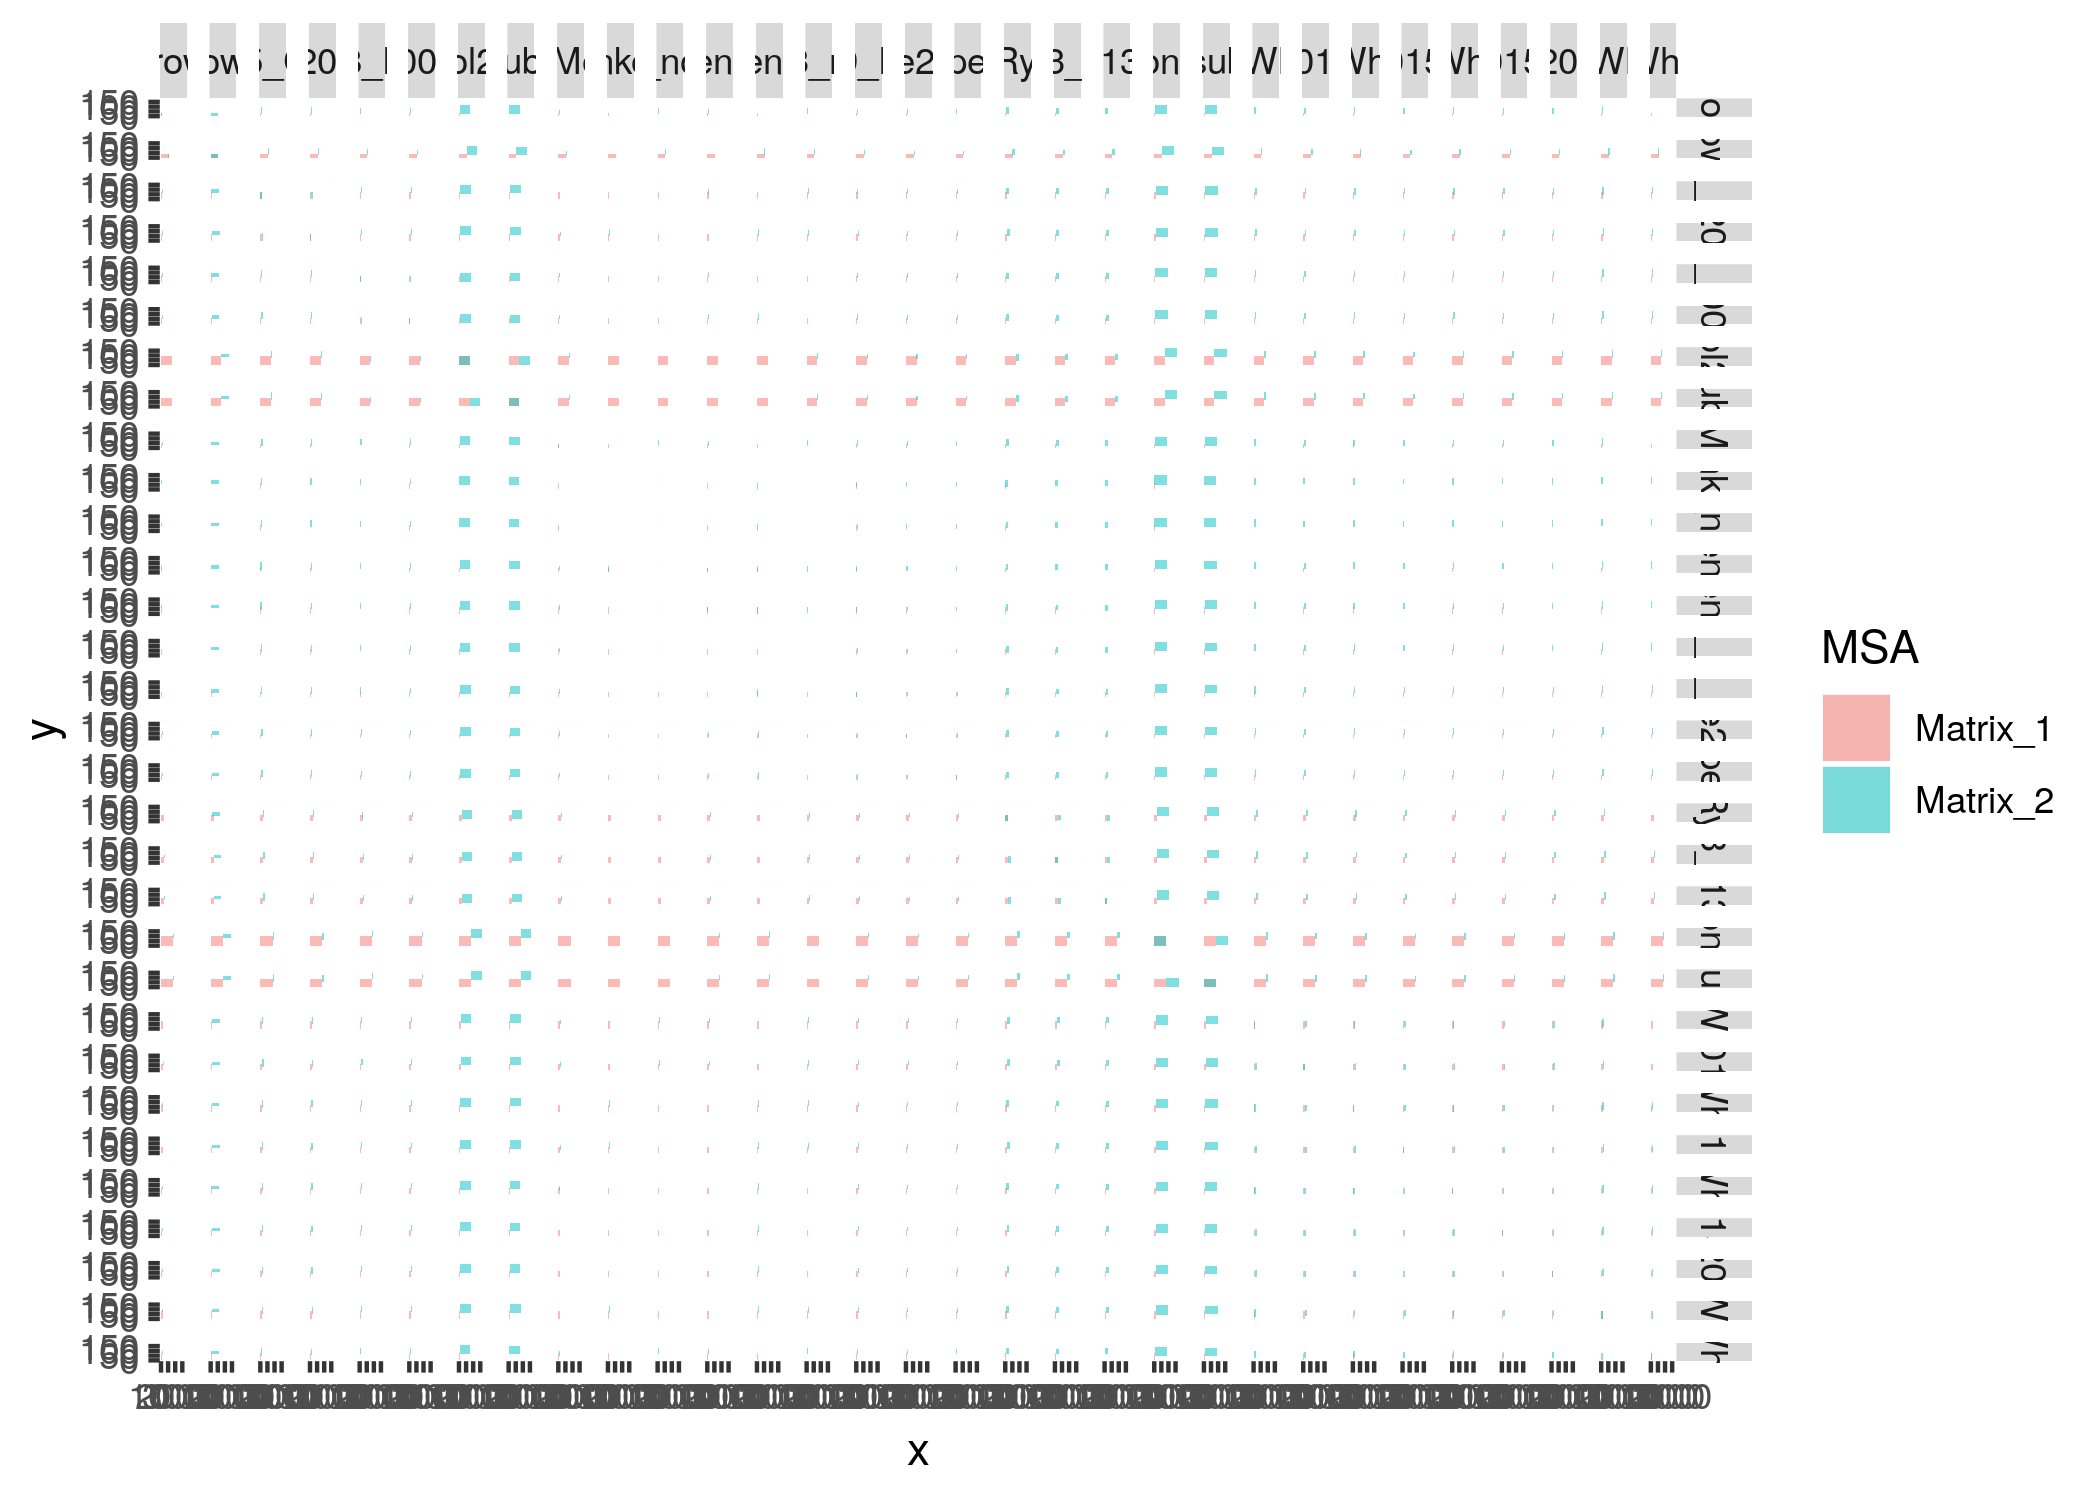
\includegraphics{manuscript_files/figure-latex/matrix_overlap-1.pdf}

\textbf{Fig. 2.} Pairwise overlap between each of the primary matrices
considered here. Horizontal size is proportional to the number of genes
sampled, vertical size to the number of taxa sampled. The horizontal
intersection shows the proportions of shared genes, the vertical
intersection shows the proportions of shared taxa.

\hypertarget{support-for-porifera-sister-and-ctenophora-sister}{%
\subsubsection{Support for Porifera-sister and
Ctenophora-sister}\label{support-for-porifera-sister-and-ctenophora-sister}}

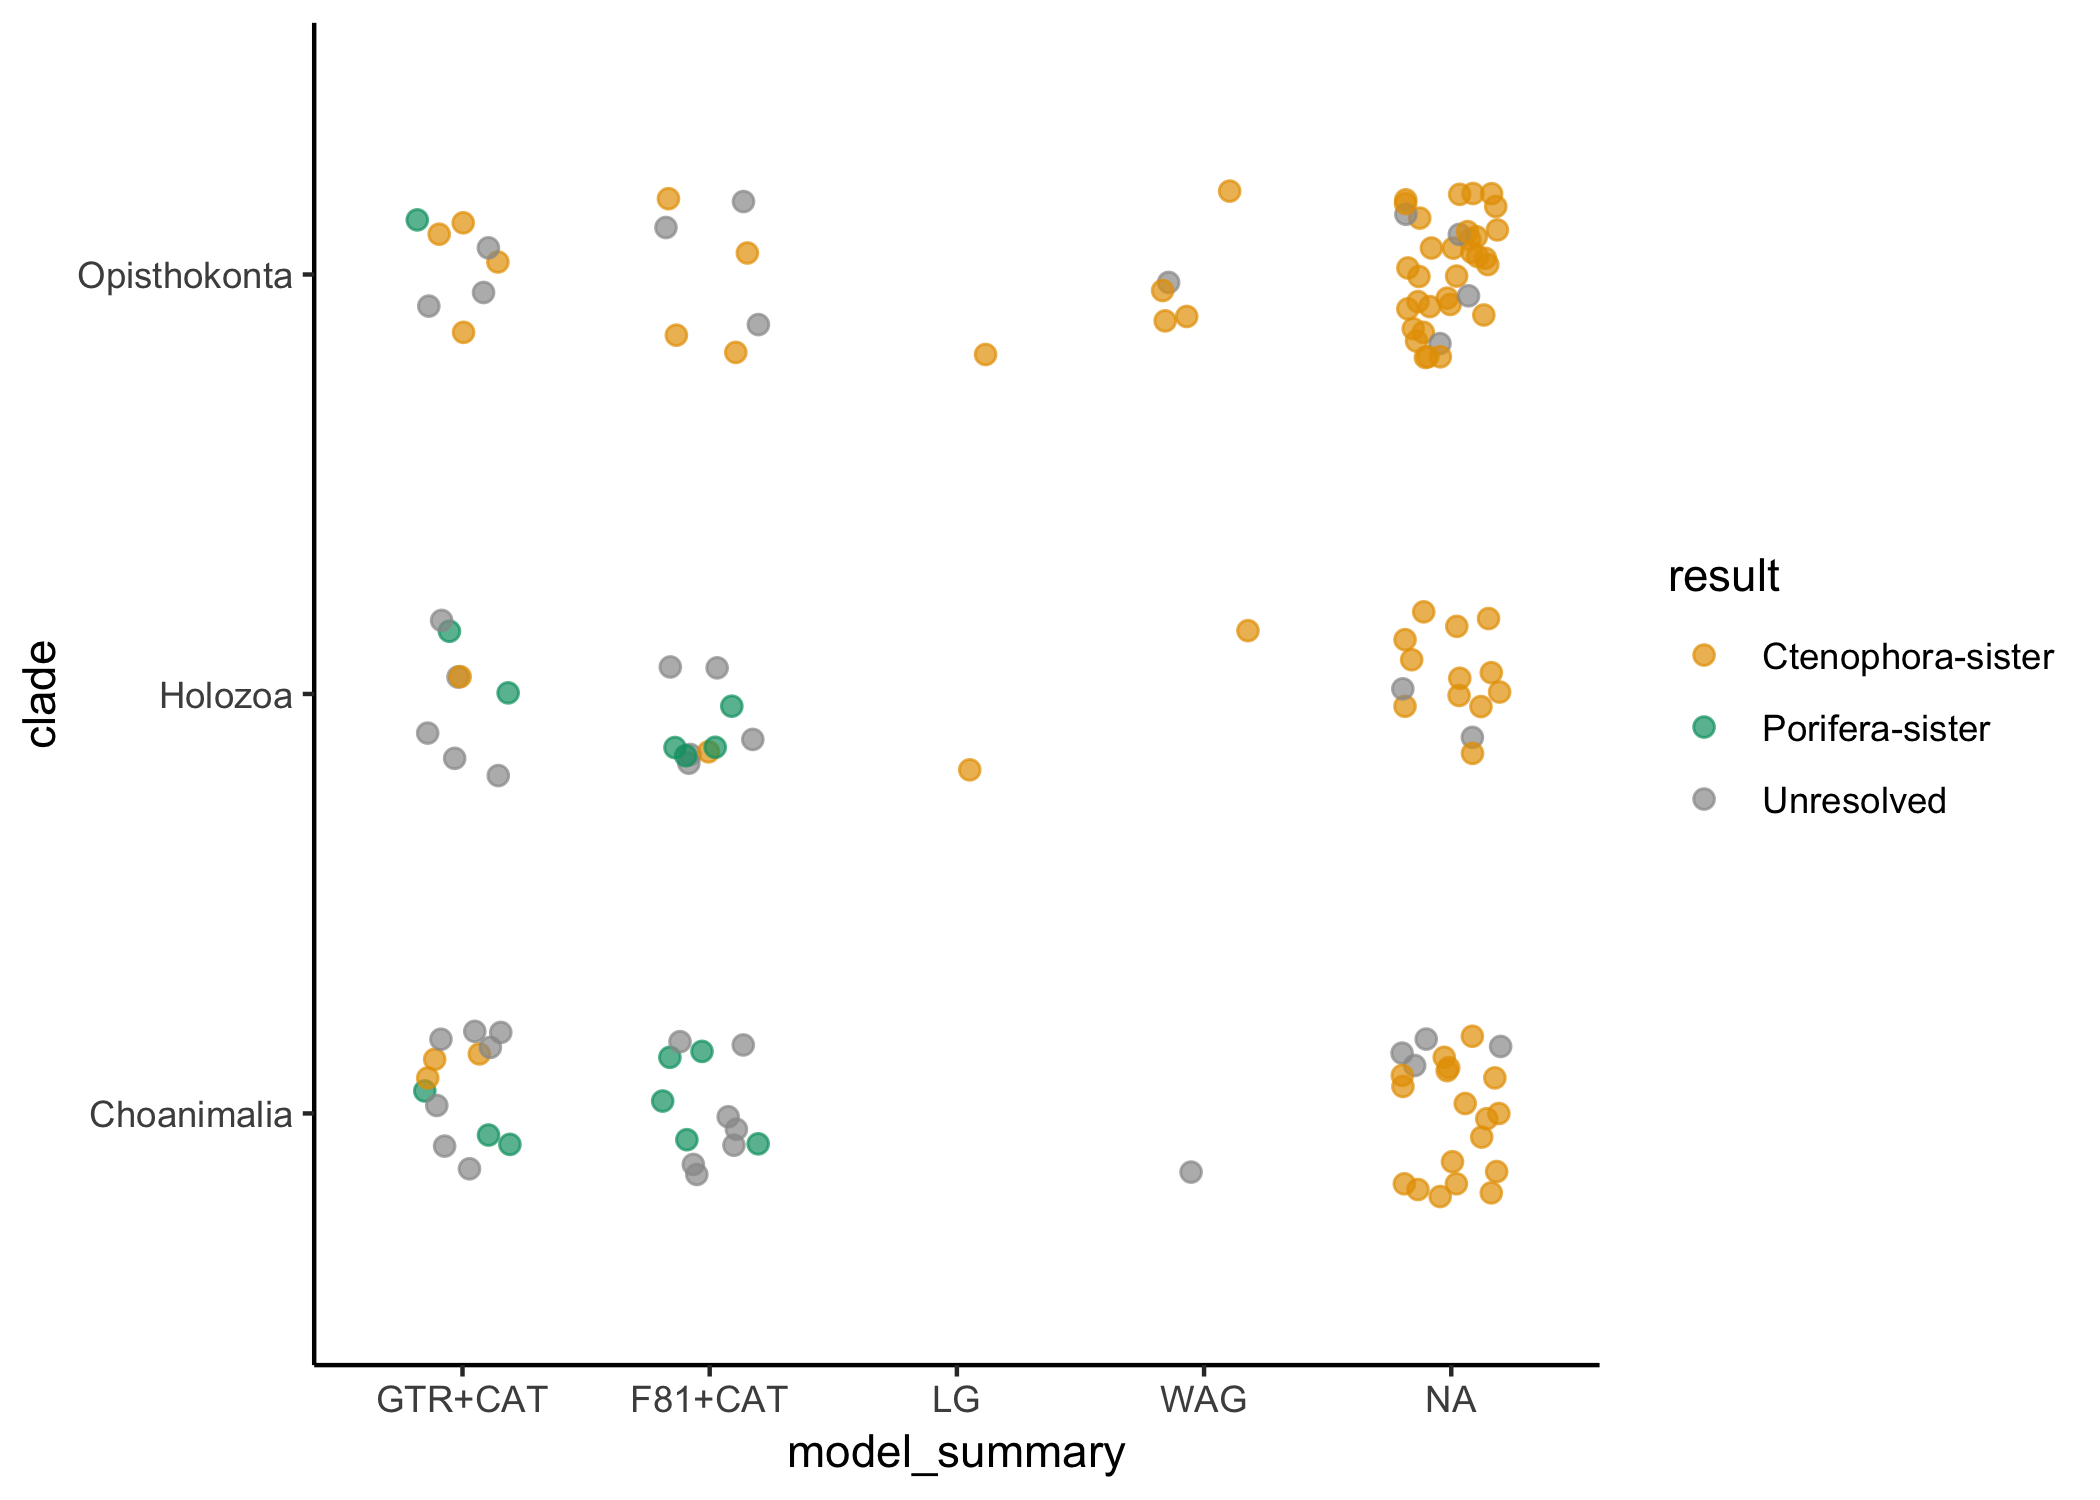
\includegraphics{manuscript_files/figure-latex/support_published_analyses-1.pdf}
\textbf{Fig. 3.} A total of 163 analyses were transcribed from the
literature (Supplementary Table 2).

Here we summarized all the 163 previous phylogenetic analyses from 15
studies (Fig. 3 and Supplementary Table 2). Among these studies, the
main conclusions of five studies strongly in favor of Porifera-sister
and 10 in support of Ctenophora-sister (Table 1). Moreover, three
studies are secondary studies without any new data matrices.
Interestingly, we found that all analyses strongly support of
Ctenophora-sister once site-homogeneous models were used, no matter what
outgroup choice, phylogenetic inference and whether data-recoding are
used. The support for Porifera-sister increases with the exclusion of
more distantly related outgroups and with the use of site-heterogeneious
CAT (Poisson+CAT or GTR+CAT) models. It should be noted that many BI
analyses with CAT model are not well resolved (either not reach
convergence or do not provide significant support for the key node of
animal evolution) mainly due to computational limits of CAT models
employed in PhyloBayes. The strong support of Porifera-sister can only
be recovered from analyses using Poisson+CAT and recoding methods with
GTR+CAT models in several matrices. Although GTR+CAT model generally has
better model adequacy than Poisson+CAT or site-homogeneous models from
previous studies\textsuperscript{6,9}, Porifera-sister is not always
supported since several analyses strongly in favor Ctenophora-sister
even with only choanofalgellates are used as outgroups (Fig. 3). Thus,
our summary of previous phylogenetic analyses strongly indicated that
the trend of the support of Porifera-sister is generally increasing with
the use of more complex CAT models and more closely related outgroups,
whereas Ctenophora-sister is supported in all other cases.

\hypertarget{new-analyses-of-published-matrices}{%
\subsection{New analyses of published
matrices}\label{new-analyses-of-published-matrices}}

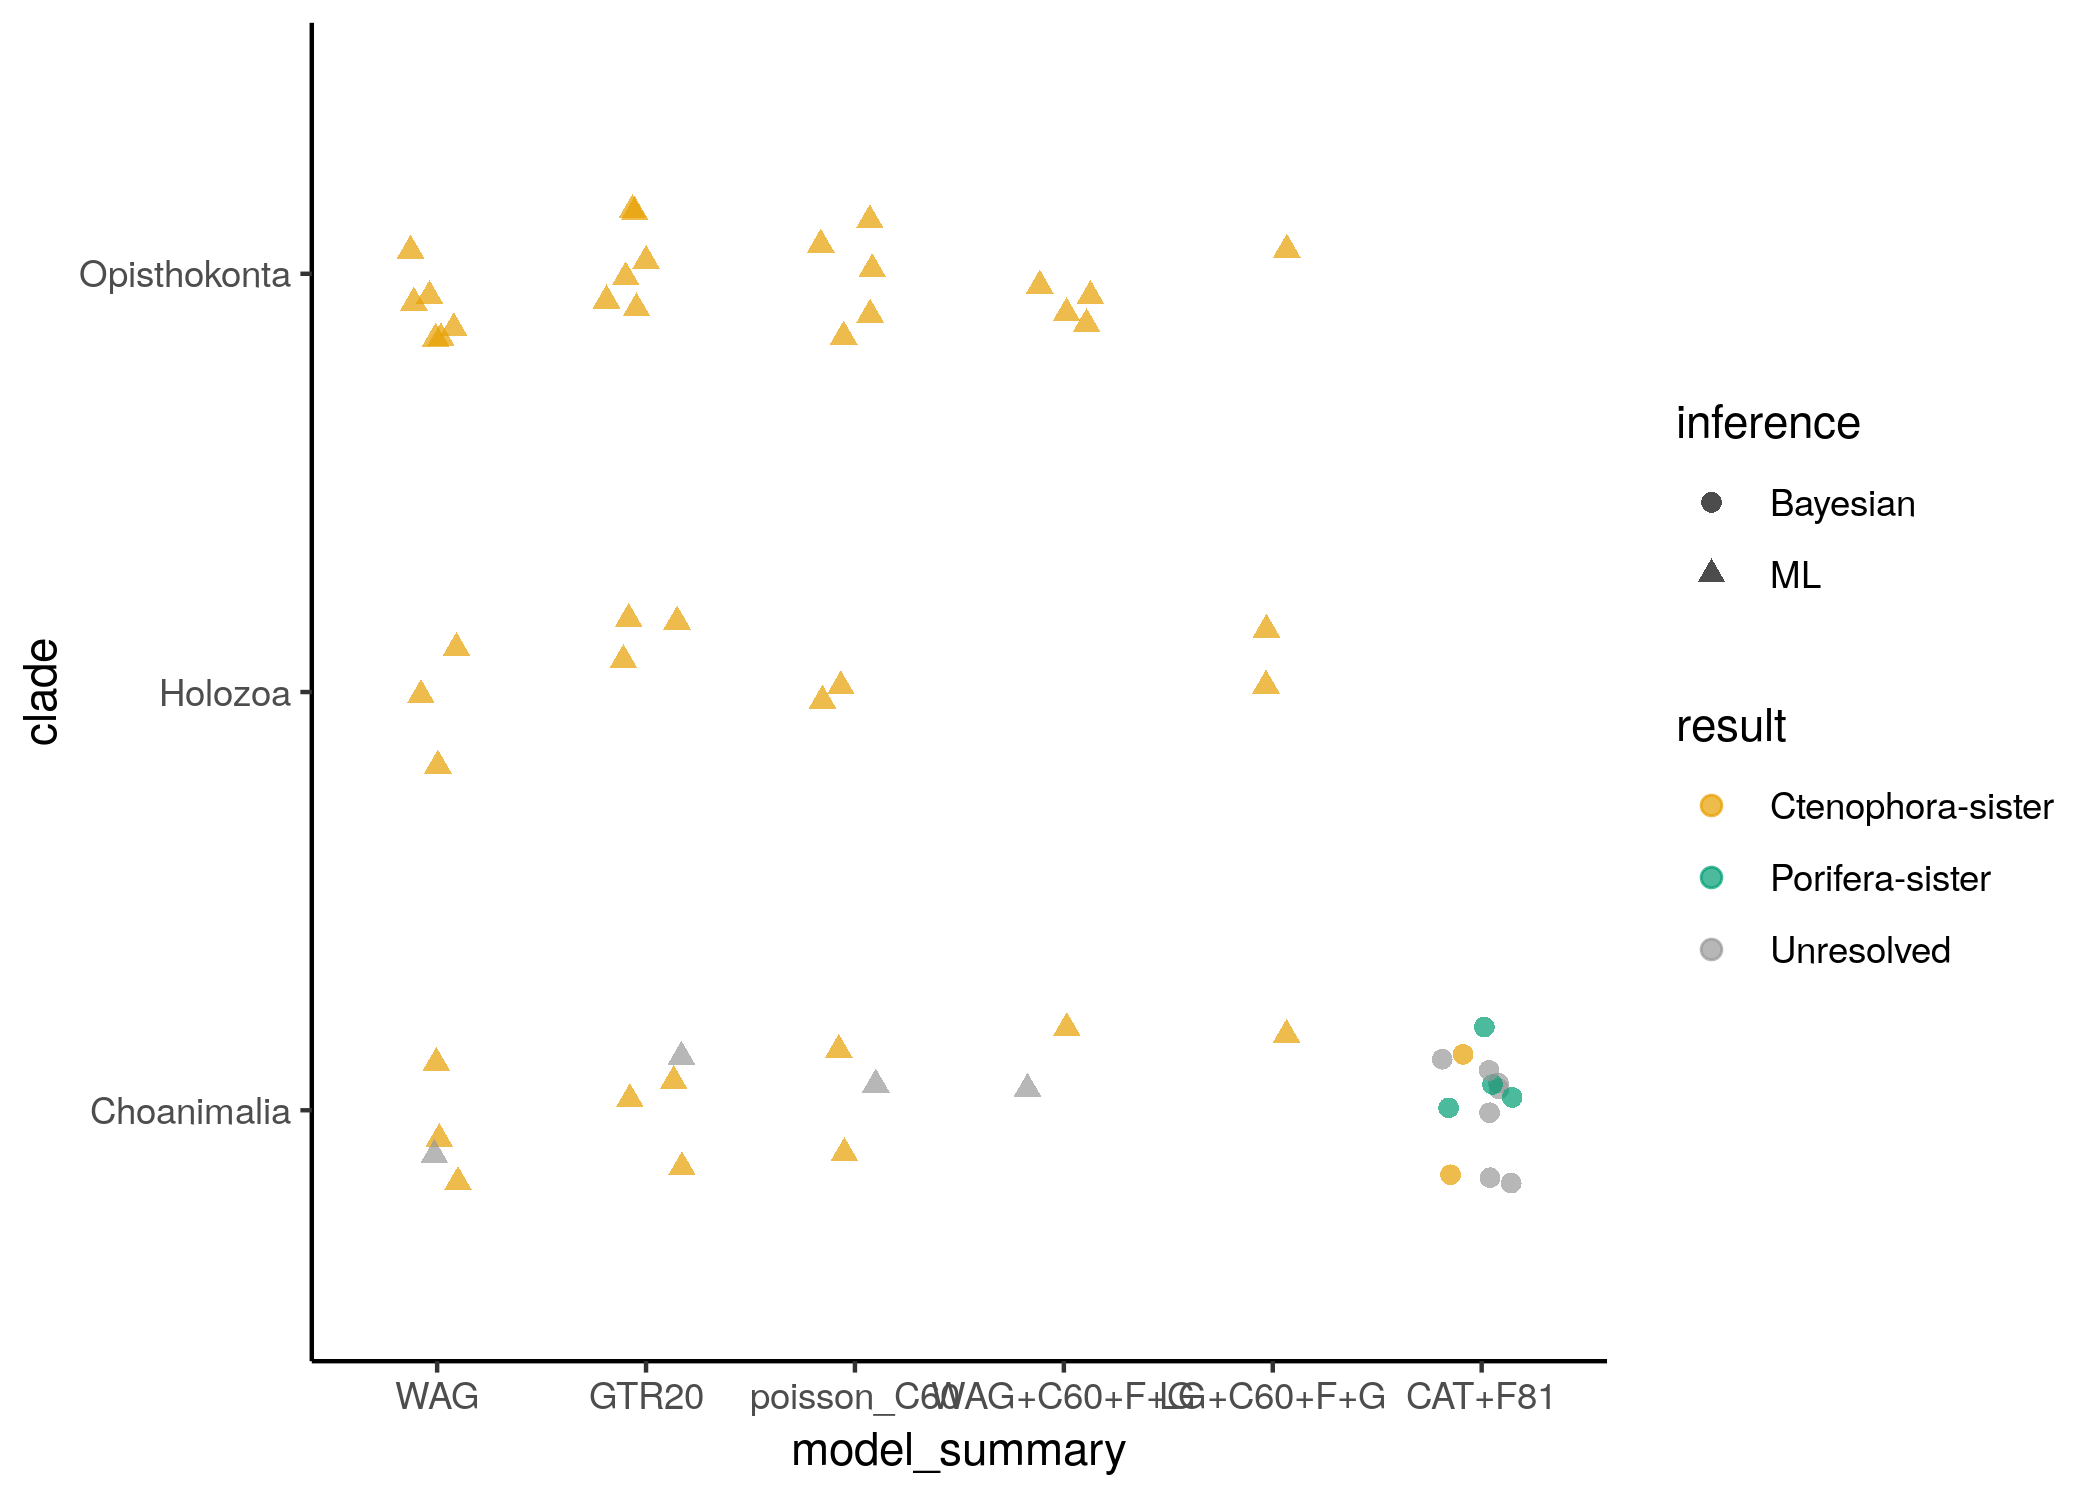
\includegraphics{manuscript_files/figure-latex/support_new_analyses-1.pdf}
\textbf{Fig. 4.} A total of 84 new phylgoenomic analyses were conducted
in this study (Supplementary Table 3).

One of the challenges of interpreting support for the placement of the
animal root is that different programs, software versions, and settings
have been used across studies, and phylogenetic analysis decisions have
been approached in very different ways. Here we first reanalyze the
primary matrices from each study under consistent conditions with
IQtree\textsuperscript{22} under a panel of evolutionary models. We
selected this tool because it has greater model flexibility,
computational time and accuracy than other tools in maximum likelihood
(ML) framework\textsuperscript{23} (Fig. 4; Supplementary Table 3).
Importantly, we also include a CAT-like, site-heterogeneous C10-C60 (C)
models\textsuperscript{24} that are implemented in both ML and Bayesian
inference (BI) framework in our analyses and it is interesting to
compare results between C60 model to CAT models since it has never been
used in any matrices analyzed here.

Here we reanalyzed 17 matrices from 15 studies that are used as main
conclusions from their original paper (Table 1). We also progressively
trimmed each data matrix with three level of outgroup choice if
applicable (Fig 1C). We first tested a variety of models for each matrix
and compared the relative fit of site-homogeneous and site-heterogeneous
C models using ModelFinder\textsuperscript{25} in IQtree (except only
LG+C60 models are used in 3 large matrices). We found in all cases,
WAG/LG+C60 models fit these matrices better than the site-homogeneous
models under BIC criteria and we then inferred support under the
best-fit model from IQtree (Extended Data Table 1). It should be noted
that we didn't include GTR+C models in model testing since it is
computational too expensive. The GTR+C models requires to estimate up to
over 10,000 (e.g.~GTR+C60 contains 234*60 parameters) free parameters
inferred from matrices, whereas only several hundred parameters needs to
estimate in site-homogeneous + C models. We then analyzed every matrix
under a panel of standard site-heterogeneous and site-homogeneous
models, including WAG, GTR and Poisson+C60. Moreover, we also used the
best-fit model identified above with the removal of all distantly
related outgroups and only include Choanoflagellata as outgroups.
Interestingly, with the exception of Moroz2014\_3d and all Nosenko2013
matrices that supports neither Porifera-sister or Ctenophora-sister, all
analysis conducted herein in IQtree strongly supported the
ctenophore-sister hypothesis, even with CAT-like, site-heterogeneous C
models with the most closely related outgroups (Fig. 4; Supplementary
Table 3).

\textbf{Extended Data Table 1.} The models selected by ModelFinder for
each matrix.

\begin{longtable}[]{@{}llll@{}}
\toprule
matrix & clade & result & model\_summary\tabularnewline
\midrule
\endhead
Borowiec2015\_Best108 & Choanimalia & Ctenophora-sister &
WAG+C60\tabularnewline
Chang2015 & Holozoa & Ctenophora-sister & LG+C60\tabularnewline
Dunn2008 & Opisthokonta & Ctenophora-sister & WAG+C60\tabularnewline
Moroz2014\_3d & Choanimalia & Unresolved & WAG+C60\tabularnewline
Nosenko2013\_nonribo\_9187 & Opisthokonta & Unresolved &
WAG+C60\tabularnewline
Nosenko2013\_ribo\_11057 & Choanimalia & Unresolved &
WAG+C60\tabularnewline
Nosenko2013\_ribo\_14615 & Opisthokonta & Unresolved &
WAG+C60\tabularnewline
Ryan2013\_est & Opisthokonta & Ctenophora-sister &
WAG+C60\tabularnewline
Whelan2015\_D1 & Opisthokonta & Ctenophora-sister &
LG+C60\tabularnewline
Whelan2015\_D10 & Opisthokonta & Ctenophora-sister &
WAG+C60\tabularnewline
Whelan2015\_D20 & Opisthokonta & Ctenophora-sister &
WAG+C60\tabularnewline
Whelan2017\_full & Holozoa & Ctenophora-sister & LG+C60\tabularnewline
Whelan2017\_strict & Choanimalia & Ctenophora-sister &
LG+C60\tabularnewline
\bottomrule
\end{longtable}

\hypertarget{comparison-of-iqtree-and-phylobayes-results}{%
\subsubsection{Comparison of IQtree and PhyloBayes
results}\label{comparison-of-iqtree-and-phylobayes-results}}

Site heterogeneity in equilibrium frequency has been a major concern in
tests of Ctenophora-sister and Porifera-sister. This has been addressed
with CAT models. IQtree provides a new family of C models that also
address site heterogeneity. Given the extensive computational cost and
concerns about overparameterization of CAT models\textsuperscript{26},
we compared iqtree C results to CAT results for a subset of matrices to
see if they give consistent results. This would be of technical interest
because it would reduce the cost of accommodating compositional
heterogeneity in future analyses. For computational efficiency, we first
only applied Poisson+CAT (Poisson+CAT) models in every matrix with
Choanoflagellata as outgroups. It should be noted that most Phylobayes
runs were converged, although several large matrices have not reached
convergence after at least a month's computational time.

Interestingly, we found strong supports for both hypotheses when using
Poisson-CAT model in Choanimalia matrices. Similar to ML analyses, we
found no strong support for either hypothesis in Moroz2013\_3d and
Nosenko2013 matrices. Consistent with previous
study\textsuperscript{27,6}, we recovered strong support of
Porifera-sister in matrices of Philippe2008, Ryan2013 and Whelan2015.
Interestingly, we also found a strong support of Porifera-sister in two
Whelan2017 matrices\textsuperscript{15} and a weaker support of
subsampled matrix of Simion2017\textsuperscript{16}. The
Ctenophora-sister were strongly supported in all other matrices. For the
matrices have conflicted results between Poisson-CAT and
site-homogeneous models, we further ran Poisson+CAT models with
inclusion of more distantly related outgroups to evaluate how outgroup
choice may affect phylogenetic inference under CAT model. We found a
weak support of Porifera-sister in Holozoa matrices and strong support
of Ctenophora-sister in all analyzed Opisthokonta matrices, indicating
that the support of Porifera-sister is increasing with inclusive of the
more closely related outgroups and CAT models. Thus, our reanalyzing
results are largely consistent with previous analyses, both suggesting
that the support of Porifera-sister is increasing with more complex
models and closely related outgroups. More importantly, our results
indicated that both model choice and outgroup sampling play a major role
in incongruent results of animal origin in several key data matrices.

\hypertarget{phylogenetic-signal}{%
\subsubsection{Phylogenetic signal}\label{phylogenetic-signal}}

The distribution of phylogenetic signal has never been quantified in
site-heterogeneous models and compared with site-homogeneous models. To
further explore the effect of model selection and outgroup choices in
animal origin, we next quantify the support of phylogenetic signal over
two alternative hypotheses (T1: Ctenophora-sister (Fig. 1A); T2:
Porifera-sister (Fig. 1B)) to three key data matrices with different
outgroup choice and models in both ML and BI framework (Fig. 5). By
calculating gene-wise log-likelihood scores between T1 and T2 for every
gene (\(\Delta\)GLS) or site (\(\Delta\)SLS) in each matrix, we found
that Ctenophora-sister had the higher proportions of supporting genes in
every analysis when using site-homogeneous models (LG or WAG in both
IQtree or PhyloBayes). Moreover, the outgroup choice has little impact
on the distribution of the support of phylogenetic signal in
sifte-homogeneous models. This finding is largely consistent with the
past study that majority of phylogenetic signal is strongly favored in
Ctenophora-sister hypothesis with site-homogeneous models in other data
matrices\textsuperscript{28}.

In contrast, the phylogenetic signal of site-heterogenous models changed
dramatically compared to the site-homogenous models. Although
Ctenophora-sister also had the higher proportions of supporting genes
with C models, we found that the phylogenetic signal decreases in many
genes using C models compared to site-homogeneous models, especially in
matrices from Ryan2013\_est that nearly 30\% of genes changed from
strong to week signal (\Delta\$lnL\textless{}2) (Fig. 5B; Supplementary
Table 4). It is not clear why the phylogenetic signal decreases in many
genes with a better fitting model as suggested by model testing in
IQtree, but our results indicated the C models lack of phylogenetic
signal compared to site-homogeneous models in the node of the root
position of animal phylogeny. In contrast to the C models, the
phylogenetic signal largely increased in Poisson-CAT models and more
importantly, the outgroup choice has a major effect of the distribution
of phylogenetic signal (Fig. 5A, C). We found that support for
Ctenophora-sister largely decreases and Porifera-sister increases
(\textasciitilde{} 20\% of sampled gene partitions) when exclusive of
more distantly related outgroups with the Poisson-CAT models
(Supplementary Table 4). The results here are further corroborated by
our phylogenomic analyses in BI, which the support of Porifera-sister
generally increases in Holozoa and Choanimalia matrices.

We also examined the level of congruence of gene partitions that are
supported in each hypothesis across different analyses in
Whelan2017\_full matrices (Fig. Extended Data Fig. 3). Consistent with
the summary of \Delta\$GLS~analysis, We found gene population that
supports in either hypothesis are largely congruent between
site-homogenous and C models, whereas little overlap was observed in
Poisson-CAT models (especially with different outgroup choice). In other
words. our results strongly indicated that the distribution of
phylogenetic signal of animal origin is largely sensitive to model
selection (site-homogeneous vs.~site-heterogeneous models). More
importantly, the site-heterogeneous CAT model is also more sensitive to
the outgroup choice than site-homogeneous and C models in
Whelan2017\_full matrices.

\includegraphics{manuscript_files/figure-latex/phylogenetic_signal-1.pdf}

\textbf{Fig.5} The distribution of phylogenetic signal for two
alternative topological hypotheses on the earliest-branching animal
lineage with different models and outgroup choice. (A). Proportion of
genes supporting each of two alternative hypotheses for each of two
alternative hypotheses for Philippe2009 matrix. (B). Proportion of genes
supporting each of two alternative hypotheses for each of two
alternative hypotheses for Ryan2013\_est matrix. (C) Proportion of genes
supporting each of two alternative hypotheses for each of two
alternative hypotheses for Whelan2017\_full matrix. The (\Delta\$GLS)
values for the genes across each data matrix are provided in
Supplementary Table 4.

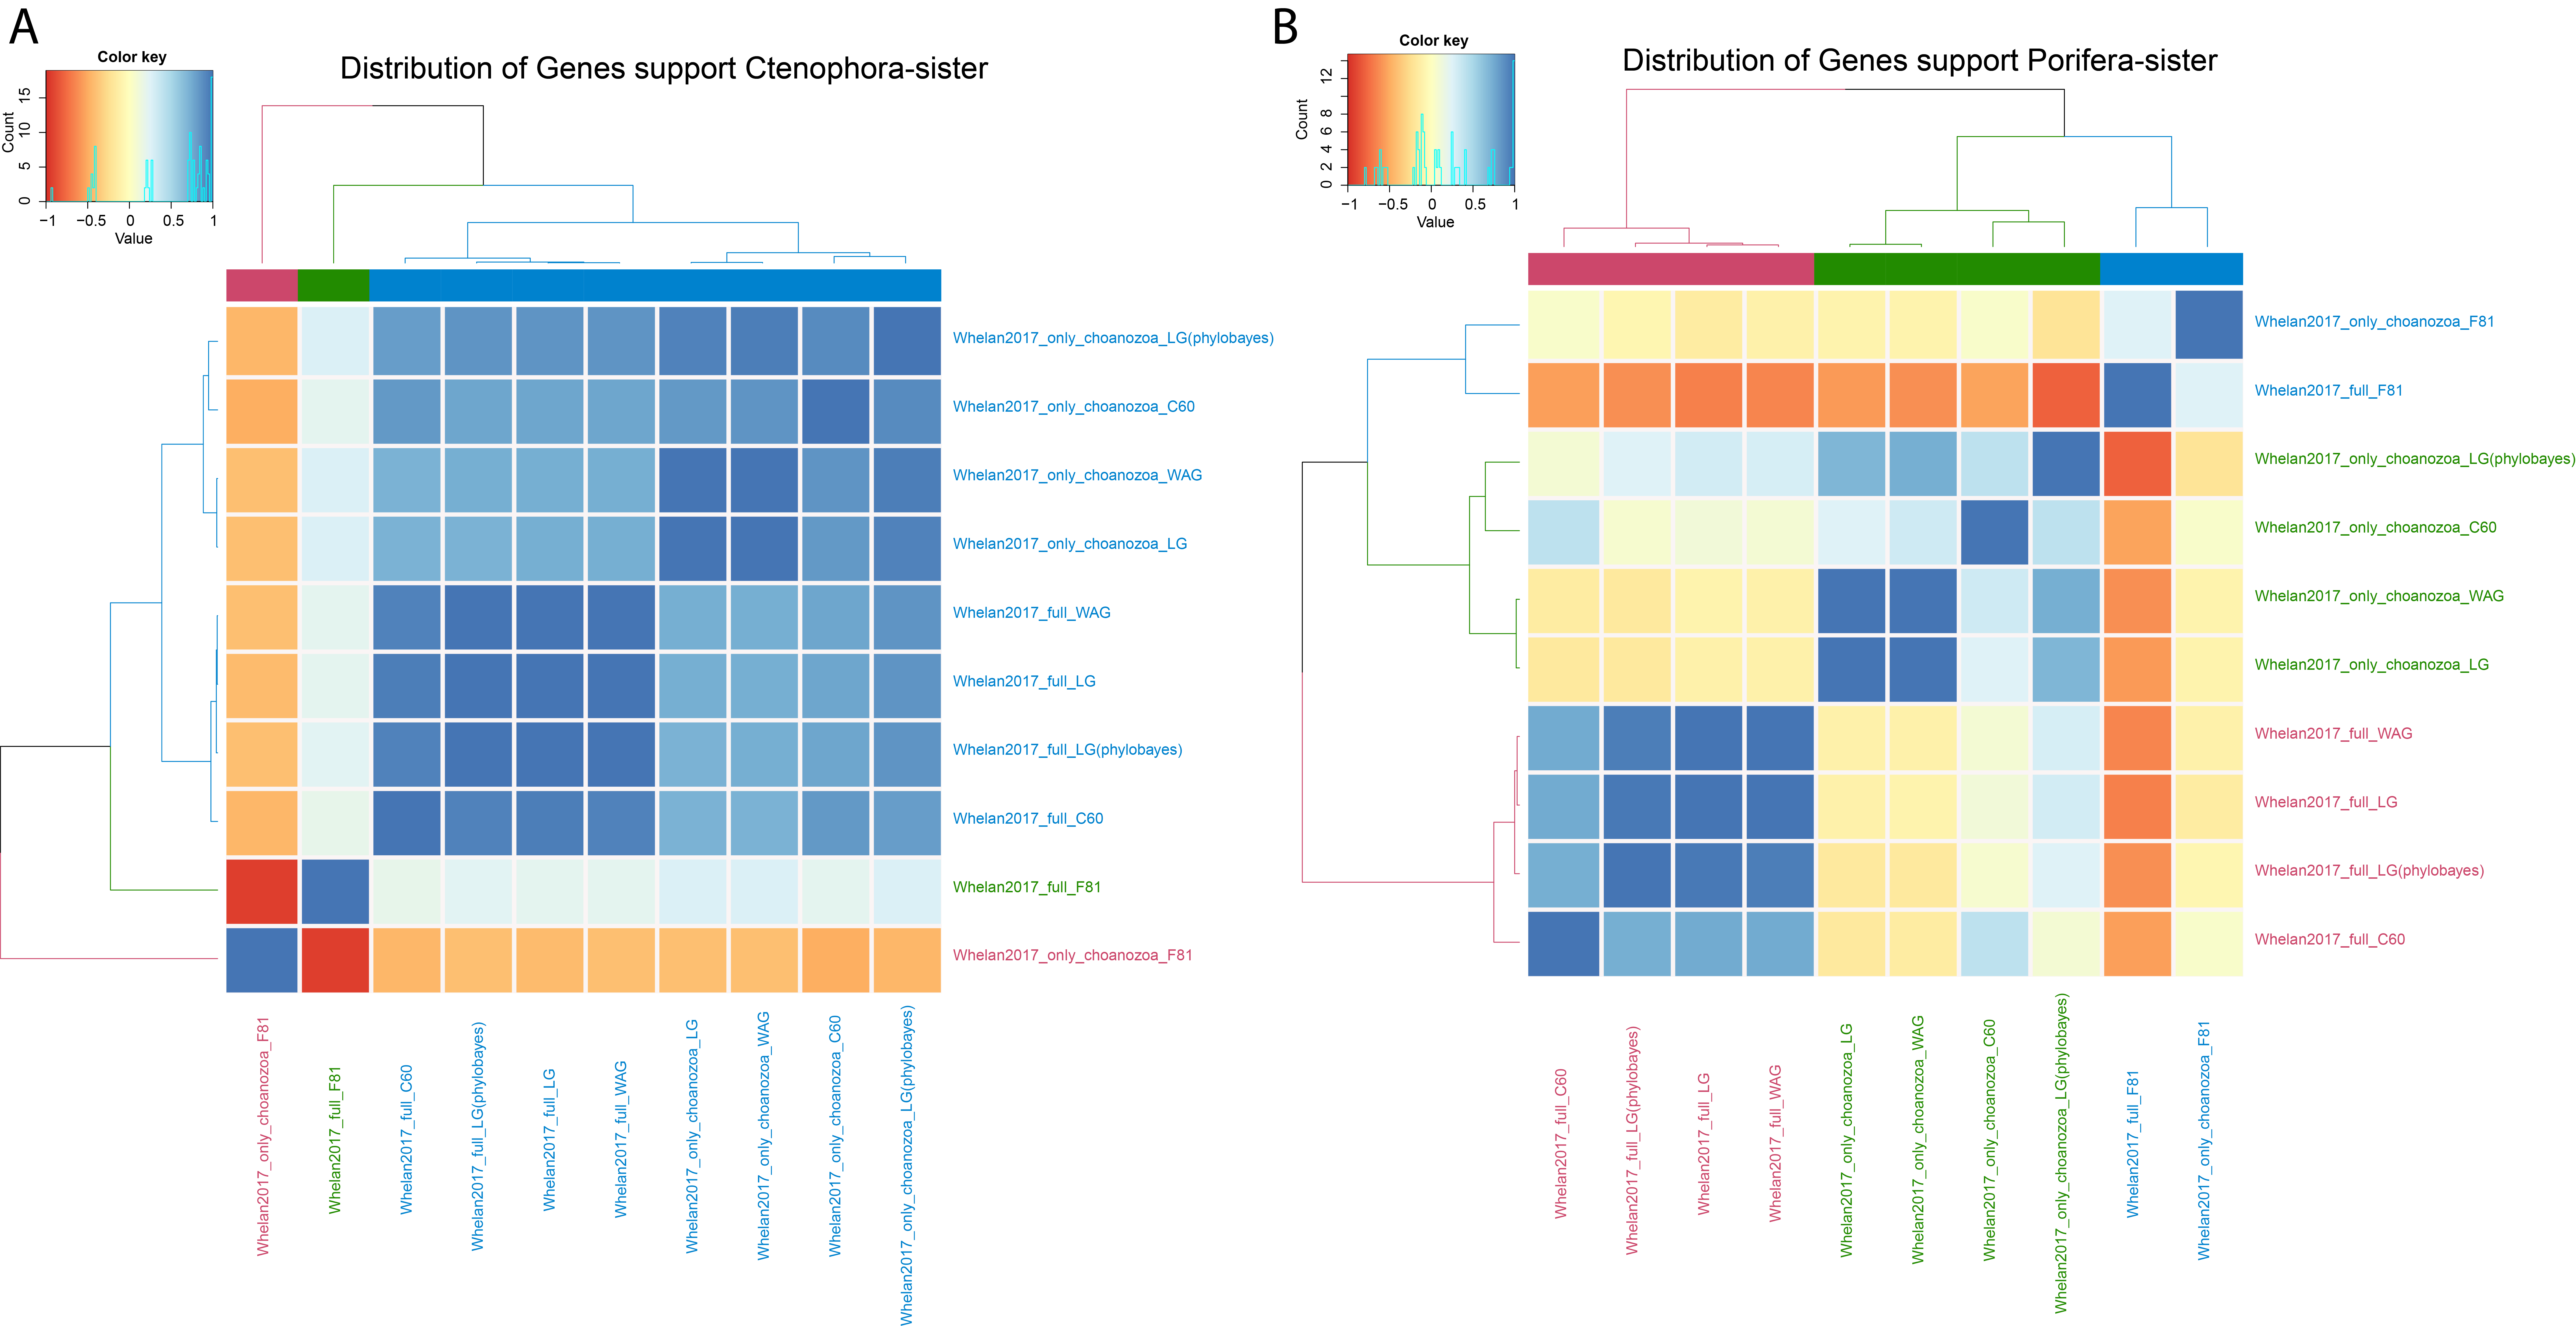
\includegraphics{figures/Figure_Pairwise_heatmap_animal_root.png}
\textbf{Extended Data Fig. 3.} Pairwise intersections of the level of
congruence of gene partitions that are supported in each hypothesis
across different analyses in Whelan2017\_full matrices calculated by
Euclidean distance. (A) Pairwise comparisons across genes that supported
Ctenophora-sister in different analyses. (B) Pairwise comparisons across
genes that supported Porifera-sister in different analyses. The color
scale indicates the Pearson correlation, where 1 is positive linear
correlation, 0 is no linear correlation, and −1 is negative linear
correlation. The pairwise intersection heatmap is generated by
Intervene\textsuperscript{29}.

\hypertarget{bias-of-data-recoding}{%
\subsubsection{Bias of data-recoding}\label{bias-of-data-recoding}}

There is growing interest in data-recoding and previous
study\textsuperscript{9} hoped that data-recoding would reduce potential
artifacts due to differences across species in amino acid frequencies.
They report that posterior predictive (PP) analyses\textsuperscript{30}
indicate 6-state recoded analyses have better model adequacy than
20-state amino acid analyses, and ``Porifera-sister was favored under
all recoding strategies'' in Whelan2015\_D20 and Chang2015 data
matrices. Here we focus on two aspects of Feuda \emph{et al.} First, we
found that many of their recoded analyses are actually unresolved
(\emph{i.e.}, without strong support for either Porifera-sister or
Ctenophora-sister), and that the analyses with the best posterior
predictive scores do not provide strong support for Porifera-sister
(Extended Data Fig. 4). Second, we created four new random recoding
schemes by shuffling the amino acids in the SR-6 scheme (see methods).
When we applied each of these randomized codes to the Whelan matrix and
analyzed them under the CAT-GTR+G model with phylobayes-mpi, we observed
similar results as for the empirical SR-6 recoding. Like SR-6 recoding,
random recoding increases support for Porifera-sister and improves the
apparent adequacy of models to explain heterogeneity of states across
taxa (PP taxon hetero mean and max, Extended Data Fig. 5). Thus, our
analyses show the impact of recoding is largely due to discarding
information, not accommodating variation in amino acid composition.
These findings indicate that it is premature to accept Porifera-sister
and reject Ctenophora-sister using data-recoding methods and recoding
can be a problematic method for addressing compositional variation (see
more detailed discussion in supplementary text).

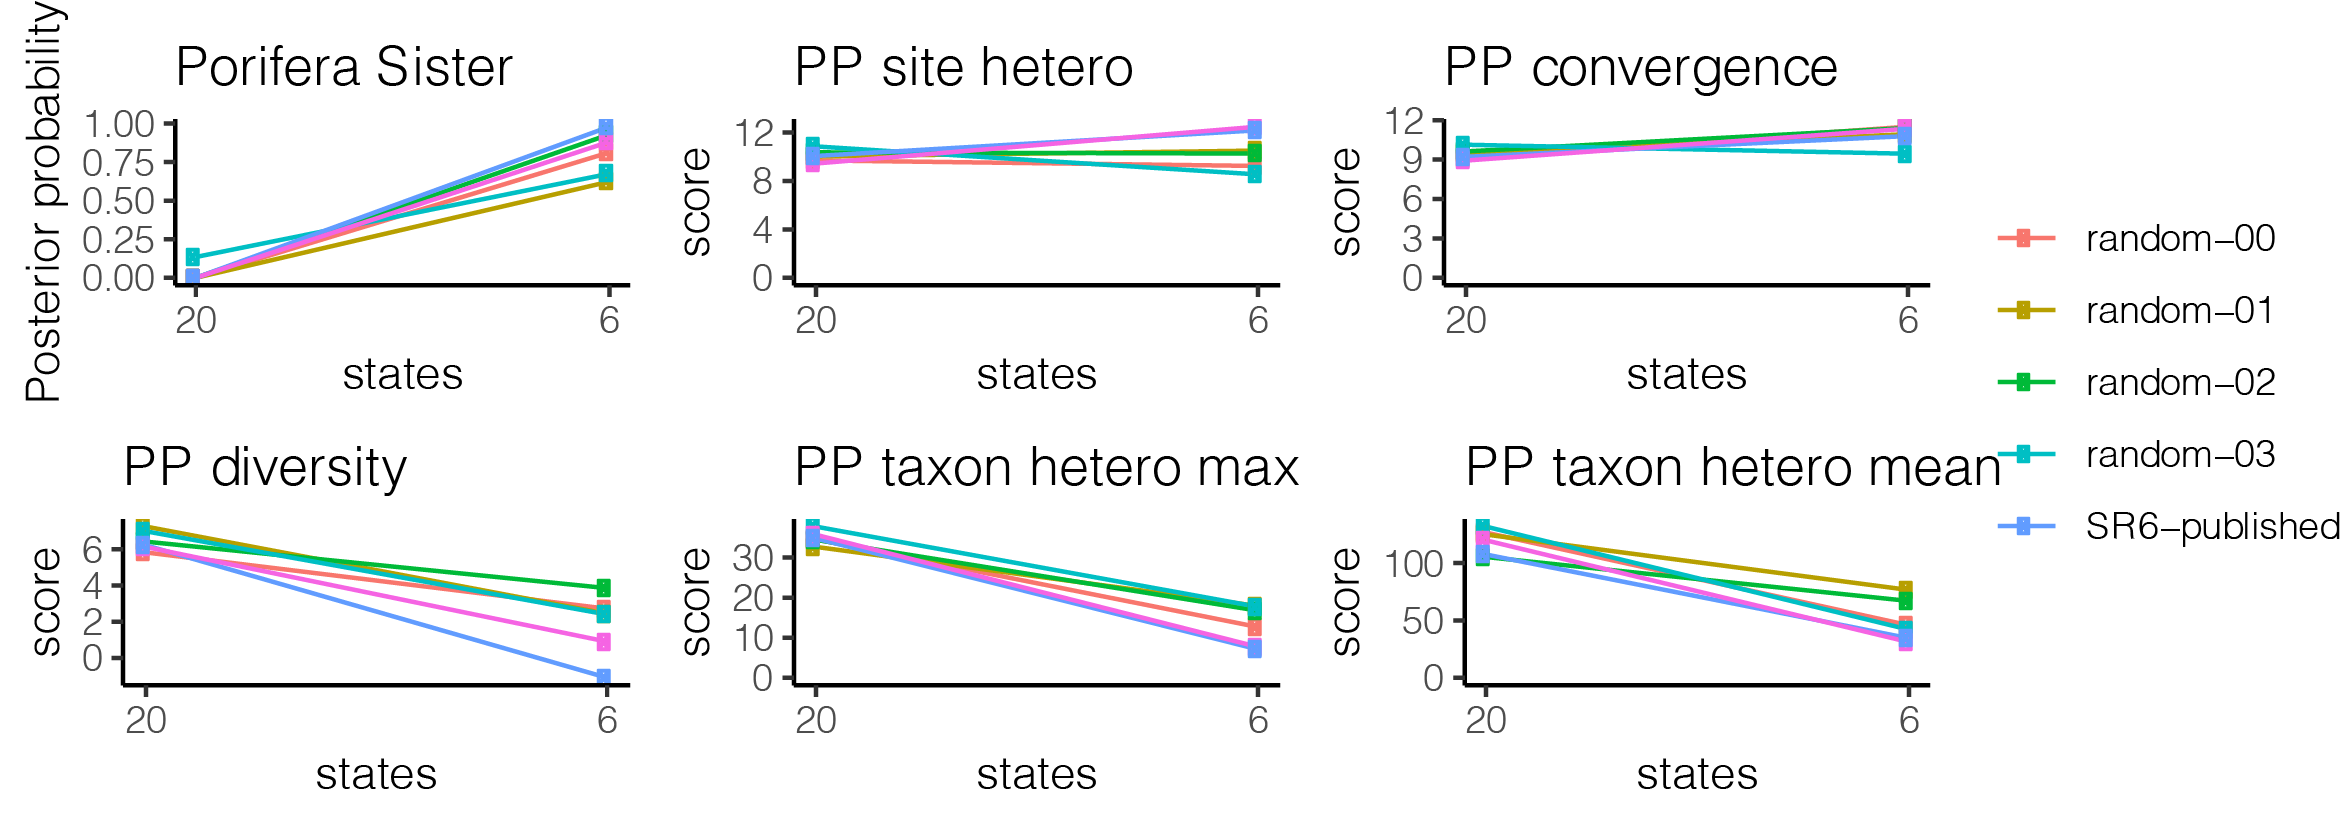
\includegraphics{figures/Figure_random_rocoding.png}

\textbf{Extended Data Fig. 4.} (A) The two alternative hypotheses for
deep animal relationships considered here. Relationships that are not
part of these hypotheses are shown as unresolved polytomies. (B) Each of
the six plots presents one statistic, which include Posterior
probability of Porifera-sister and the five Posterior Predictive (PP)
statistics considered by Feuda \emph{et al.} Within each plot, there are
six lines for six different analyses. These six analyses are the
published SR-6 analyses presented by Feuda \emph{et al.}
(SR6-published), analyses obtained by applying the same methods to the
same data to to confirm that I can reproduce their published results
(SR6-reproduced), and four analyses based on randomized recoding
matrices obtained by shuffling the SR-6 coding scheme (random-00 --
random-03). Each analysis includes results for 20 states (the raw amino
acid data, shown by the left point) and for 6 states (the 6-state
recoded data, shown by the right point). For each statistic, the results
obtained with the random recoding are similar to those of the SR6
recoding. This indicates that the impact of recoding is dominated by
discarding data when collapsing from 20 states to 6 states, not
accommodating compositional heterogeneity across lineages.

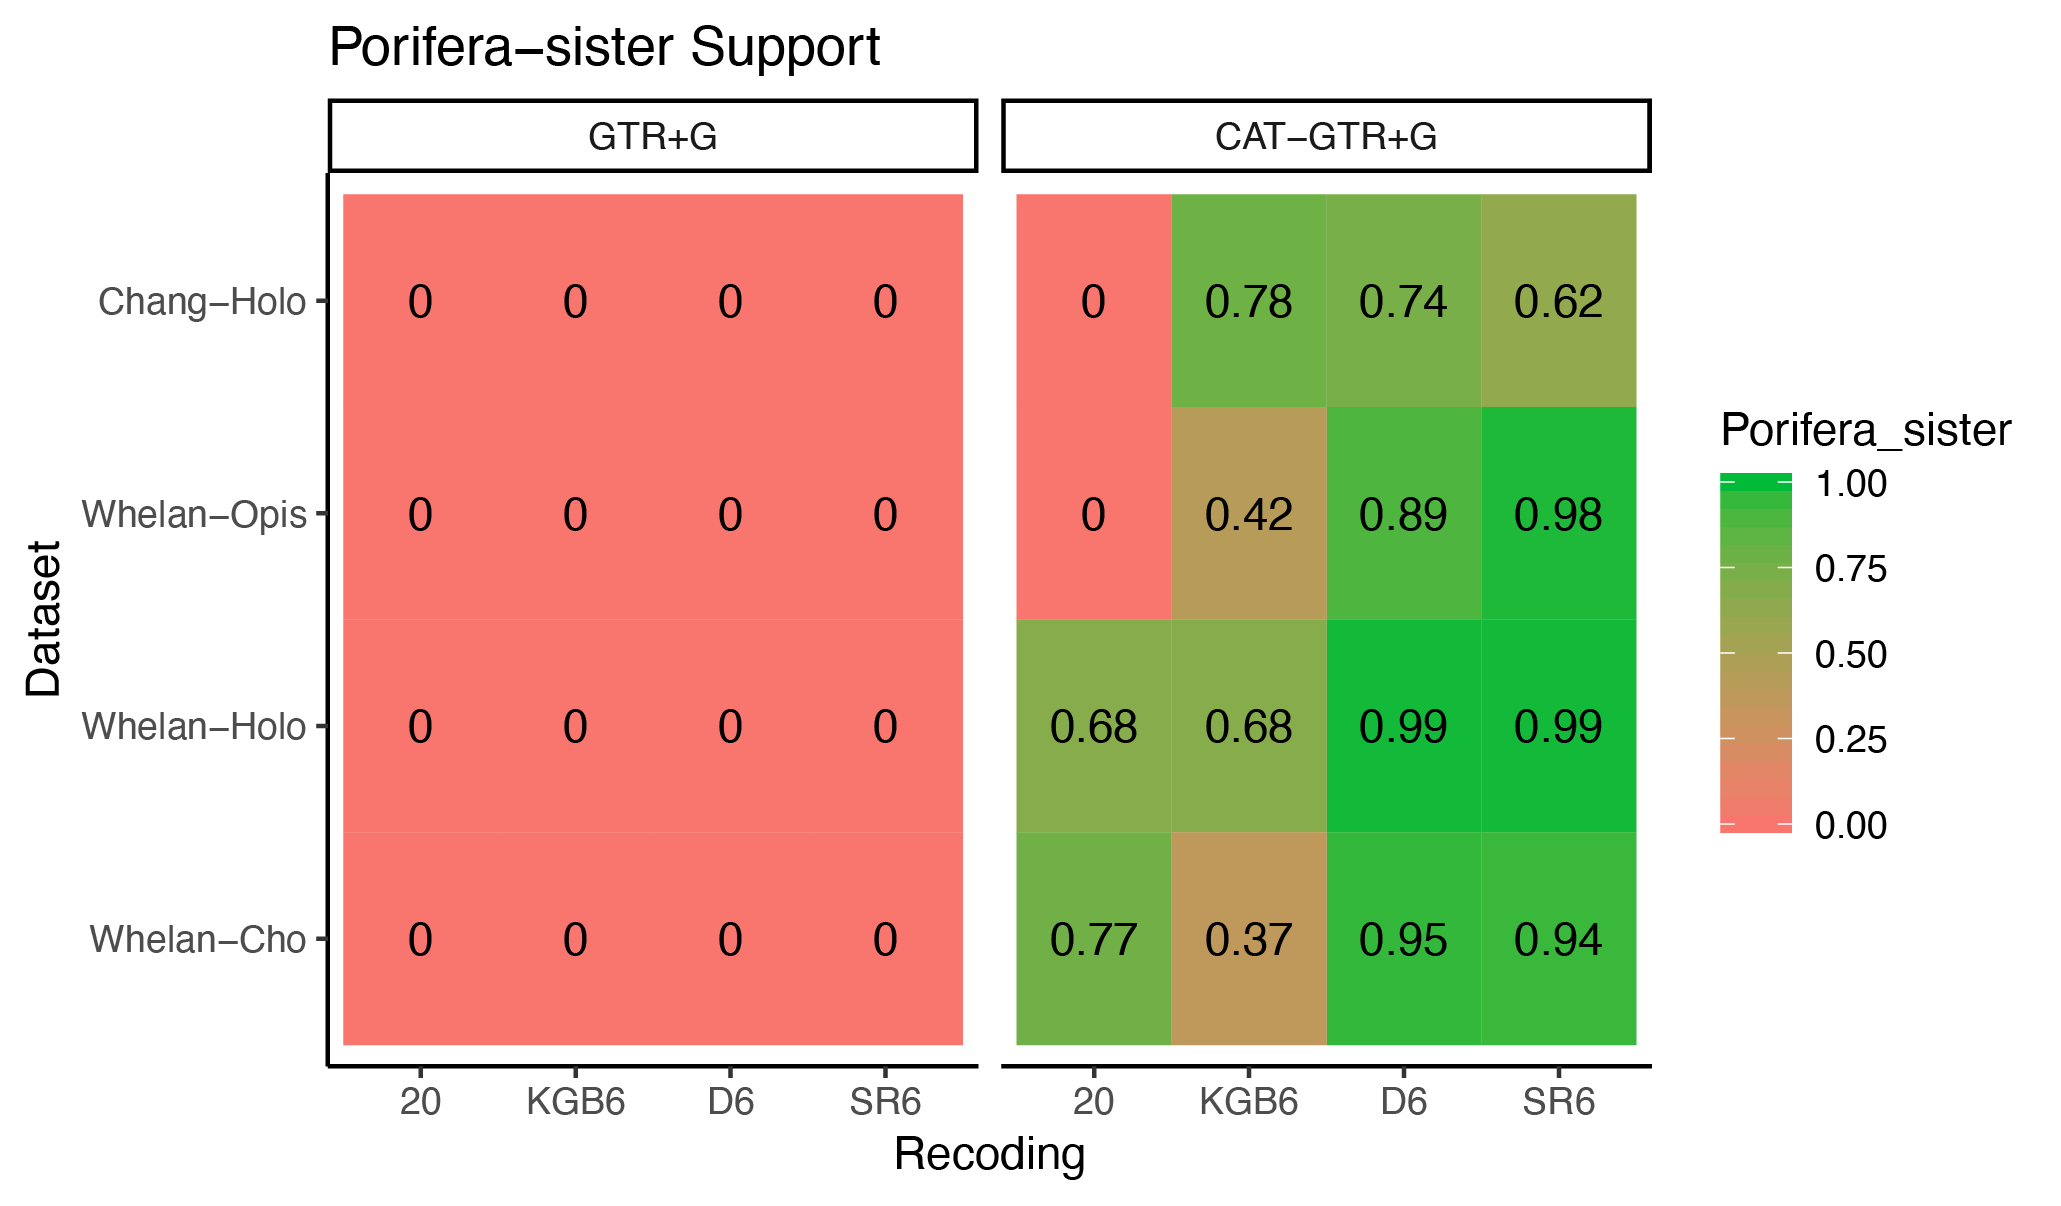
\includegraphics{figures/Figure_recoding_summary.png} \textbf{Extended
Data Fig. 6.} A graphical representation of the posterior probabilities
for the 32 analyses presented by Feuda \emph{et al.} in their Table 3.
Cells are color coded by whether posterior probability is \textgreater{}
95 for Porifera-sister, \textgreater{} 95 for Ctenophora-sister, or
neither (unresolved). Posterior predictive (PP) statistics were
estimated for the 16 analyses in the top two rows of this figure (the
Chang and full Whelan matrices), but not the bottom two (the Whelan
matrices with reduced outgroup sampling).

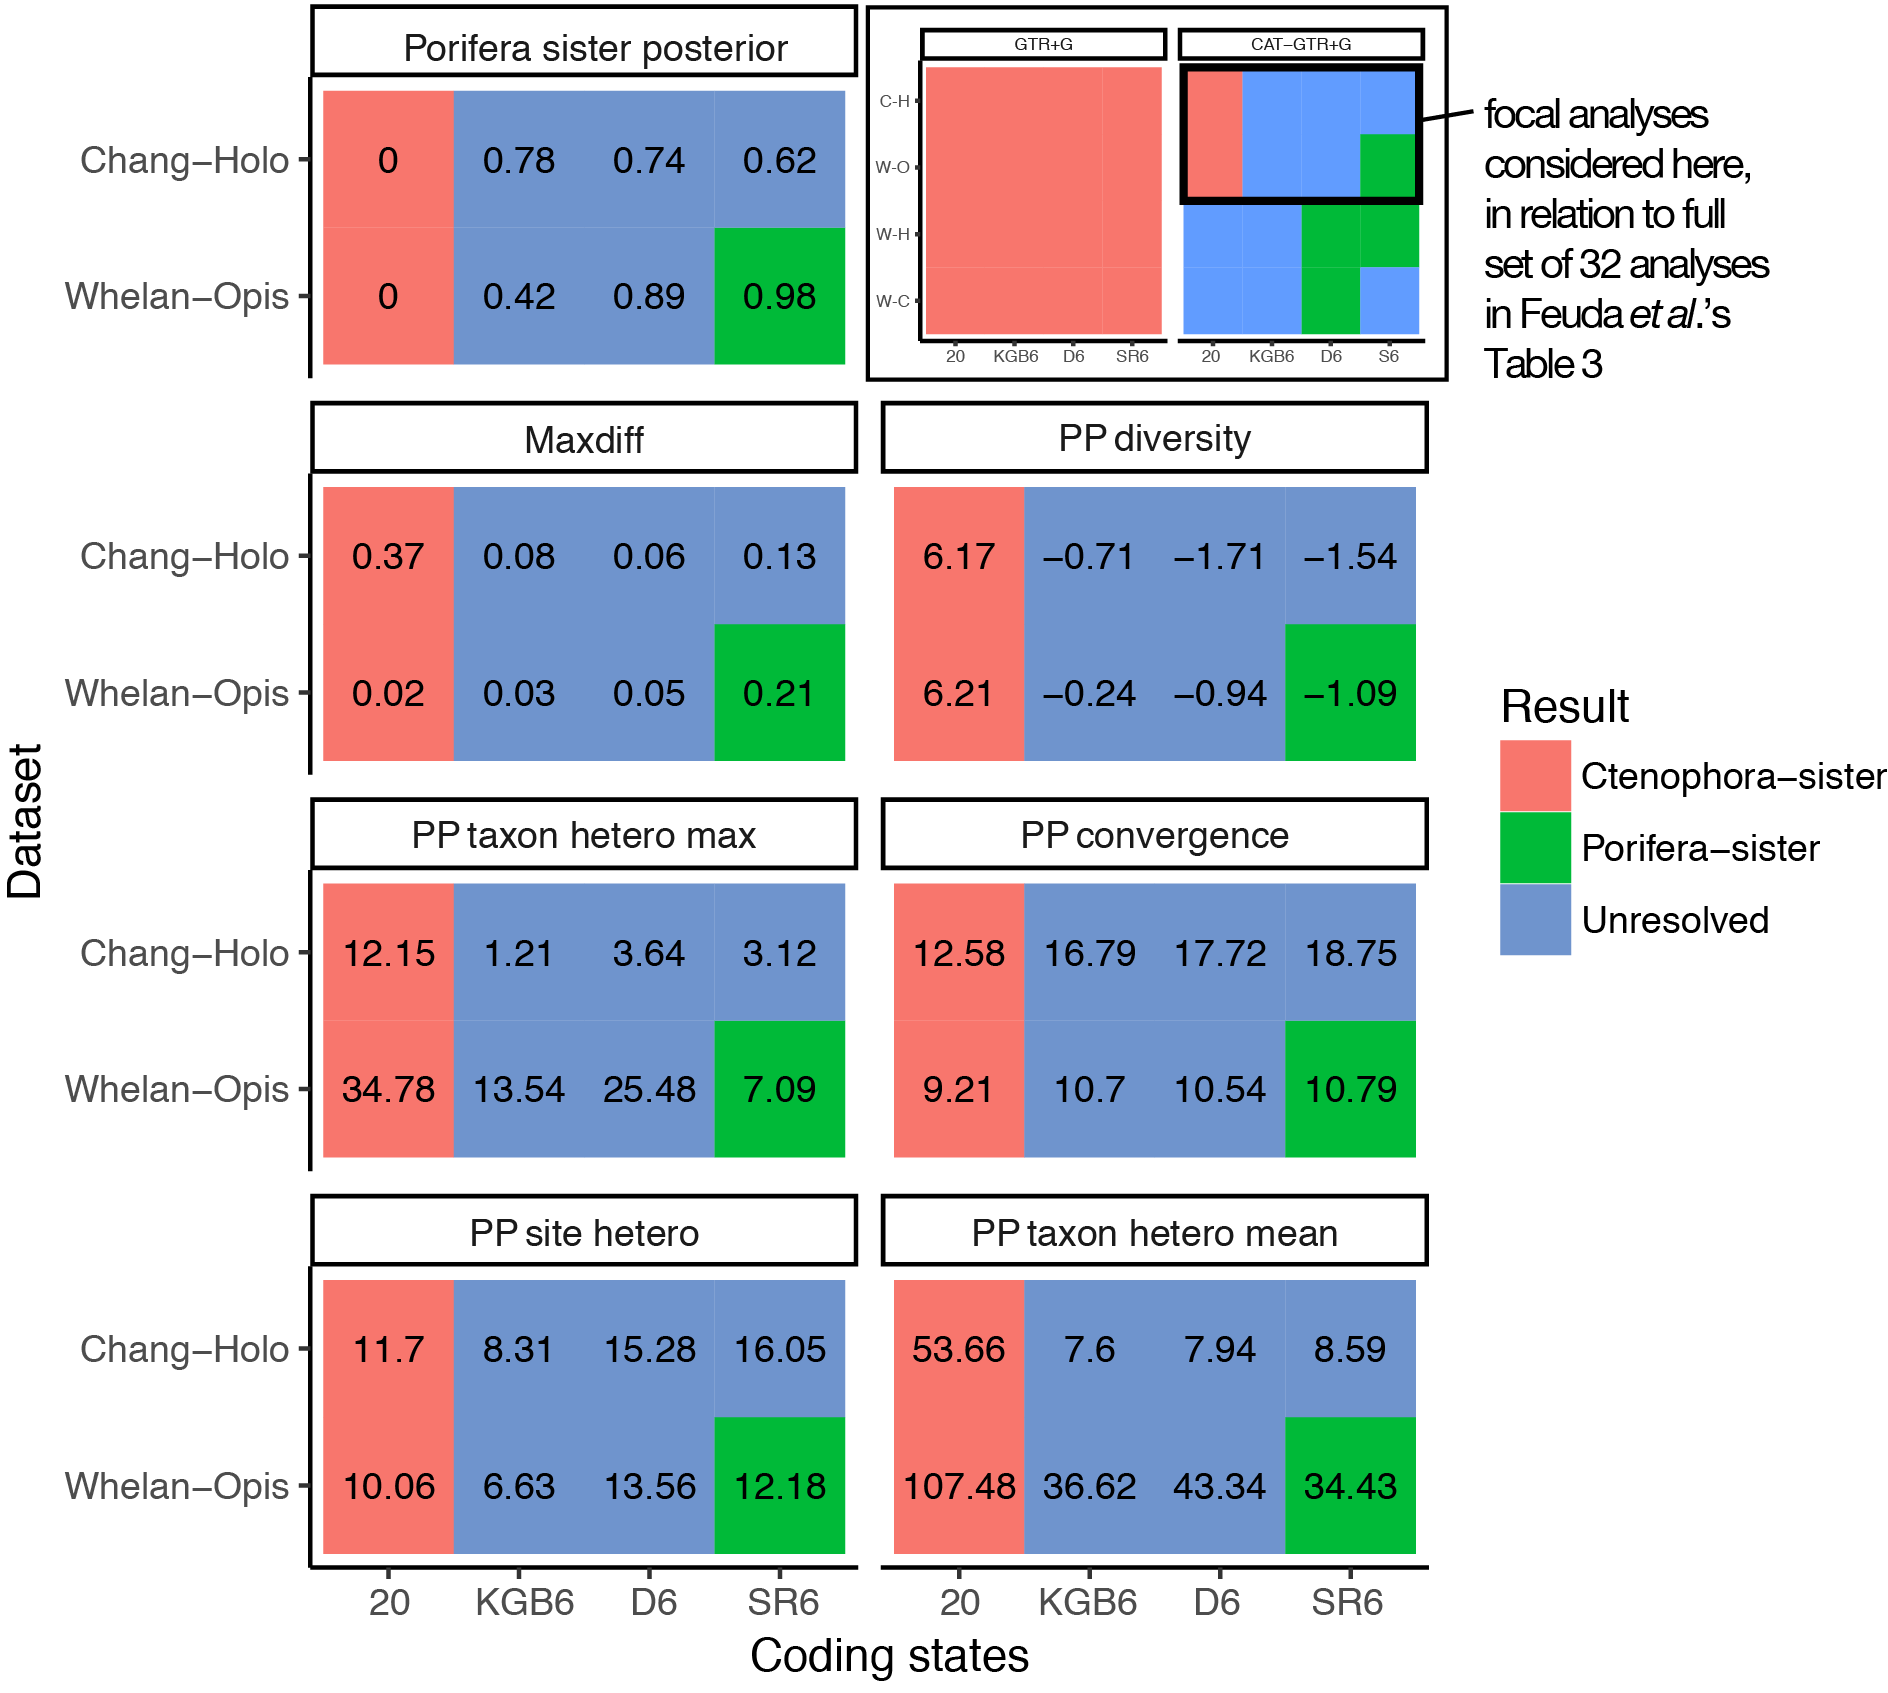
\includegraphics{figures/Figure_recoding_pp.png}

\textbf{Extended Data Fig. 5.} The subset of eight CAT-GTR+G analyses
with posterior predictive (PP) scores that is the focus of Feuda
\emph{et al.}'s primary conclusions. These are a subset of the 32
analyses presented in their Table 3 and graphically here in the upper
right pane. The eight analyses are for two datasets (Chang and Whelan)
and four coding schemes. The coding schemes are the original 20 state
amino acid data, and three different six state recodings that group
amino acids based on different criteria: KGB6, D6, and SR6. Cells are
color coded as in Supplemental Fig XXRecoidng\_summary. Only one of
these analyses, the SR6 coding of the Whelan matrix, has \textgreater{}
95 support for Porifera-sister. The 20-state and 6-state points on the
plots in Fig XXRecoidng\_summary of the main text correspond to the 20
and SR6 Whelan cells shown here. The presented statistics for these
cells are posterior probability of Porifera-sister, Maxdiff (with lower
scores indicating better convergence of runs), and five posterior
predictive statistics (where lower absolute value indicates better model
adequacy). The only one of these eight analyses that provides strong
support for Porifera-sister is not the most adequate analysis by any of
the posterior predictive scores, and showed the poorest convergence
according to Maxdiff.

\hypertarget{the-current-state-of-understanding-and-future-direction}{%
\subsection{The current state of understanding and future
direction}\label{the-current-state-of-understanding-and-future-direction}}

Resolving the root position of animal phylogeny that diverged
\textasciitilde{} 650 million years ago has proven difficult, even with
large genome-scale phylogenomic data matrices. By synthesizing all past
phylogenomic studies and perform new analyses to characterize difference
between studies, we found the support of Porifera-sister can only be
recovered by more complex CAT models with the most closely related
outgroups, and Ctenophora-sister in all other cases. Three factors
contribute significantly to the previous incongruent results based on
our analyses. First, the overlap of gene sampling and matrix is
extremely low across different studies, leading to the difficult of
directly compare the results across different studies. Second, the
distribution of phylogenetic signal are largely varied between
site-homogeneous and site-heterogeneous models. More importantly,
site-heterogeneous models are also more sensitive to outgroup choice
than site-homogeneous models, leading to different results even with the
same data matrix with different outgroup choice. Third, we demonstrated
that the support of Porifera-sister by data-recoding methods is
potentially resulted by data reduction, not accommodation of
compositional heterogeneity across species. Thus, the recovery of
Porifera-sister needs more constraints than Ctenophora-sister. Rather
than embracing one hypothesis over another, our results provide an
integrative overview of the challenge and uncertainty related to the
origin of animals.

\hypertarget{future-direction}{%
\subsection{Future direction}\label{future-direction}}

Many key positions of animal phylogeny can be reconstructed by
increasing genome-scale data within a phylogenomic framework, although
new challenges have also arised. Overcoming the challenges to inferring
the earliest diverging animal lineage is particular difficult and here
we discuss the several aspects that will help to improve our
understanding of animal evolution. First, a broader sampling of
high-quality sponge and ctenophore genomes are needed to shorten the
long branch since they are among the longest branches in the animal
phylogeny (currently only 2 ctenophore and 3 sponge genomes are
available). Second, accurate reconstruction of orthologs and a consensus
analytical strategy should be formalized with investigators to improve
communications and reproducibility of phylogenetic
workflow\textsuperscript{31}. Last, we also hope that the work we have
conducted here, including consolidating all the datasets in one place
with consistent formats and species names, will enhance the technical
value of this interesting question to methods-focused investigators that
look to develop and evaluate methods or evolutionary models to address
this difficult phylogenetic problem. More importantly, we also hope all
investigators critically evaluate the competing hypotheses without bias
instead of showing preferences to one hypothesis over as a priori due to
historical reasons or previous work. Finally, other sources of evidence
may also provide important insight to animal origin, including
morphological characters\textsuperscript{32,33} and fossil
records\textsuperscript{34}. We hope the future breakthroughs that will
allow us to move the field forward and a consensus viewpoint of early
animal evolution will be reached in the coming years.

\hypertarget{methods}{%
\subsection{Methods}\label{methods}}

All files and bioinformatic commands associated with this analysis are
available at \url{https://github.com/caseywdunn/animal_root}

\hypertarget{data-selection-and-wrangling}{%
\subsubsection{Data selection and
wrangling}\label{data-selection-and-wrangling}}

We retrieved matrices from each publication (Table 1), storing the raw
data in this manuscript's version control repository. We manually edited
some minor formatting to make the batch processing of the matrices
\emph{en masse}, e.g.~standardizing the formatting of charset blocks.
All changes made are tracked with git.

\hypertarget{matrix-comparison-and-annotation}{%
\subsubsection{Matrix comparison and
annotation}\label{matrix-comparison-and-annotation}}

\hypertarget{taxon-name-reconciliation}{%
\paragraph{Taxon name reconciliation}\label{taxon-name-reconciliation}}

We programmatically queried the NCBI Taxonomy database to standardize
names of samples in each matrix. We also use a table where manual
entries were needed (Supplementary Table 5,
reconciliation/taxonomy\_info/manual\_taxonomy\_map.tsv), e.g.~authors
of original matrix indicate species name in original manuscript. For a
table summarizing all samples and their new or lengthened names, see
Supplementary Table 6 (reconciliation/taxonomy\_info/taxon\_table.tsv).

\hypertarget{sequence-comparisons}{%
\paragraph{Sequence Comparisons}\label{sequence-comparisons}}

Using the partition files for each matrix, we isolated each sequence for
each taxon from each partition. Because many of the matrices had been
processed by the original authors to remove columns that are poorly
sampled or highly variable, these matrix-derived sequences can have
deletions relative to the actual gene sequences.

We used DIAMOND\textsuperscript{35} to compare each sequence to all
others using default diamond Blastp parameters. We further filtered
DIAMOND results such that we retained hits for 90\% of partitions
(pident \textgreater{} 78.0, eValue \textless{} 1e-15, no
self-\textgreater{}self). We ran BUSCO with default parameters for all
sequences against the provided metazoa gene set. We also ran a BLAST+
blastp search against the SwissProt\textsuperscript{21} database,
filtering such that we retain at least one hit for \textasciitilde{}97\%
of partitions (pident \textgreater{} 50.0, eValue \textless{} 1e-15).

\hypertarget{partition-network}{%
\paragraph{Partition Network}\label{partition-network}}

We used the sequence similarity comparisons described above to compare
partitions.

We constructed a network with Python and NetworkX\textsuperscript{36}
v2.2 where each node is a partition and each edge represents a DIAMOND
sequence-to-sequence match between sequences in the partitions. We
extracted each connected component from this network. We further split
these components if the the most connected node (i.e.~most edges) had
two times more the standard deviation from the mean number of edges in
the component it is a member of and if removing that node splits the
component into two or more components. We then decorated every node in
the partition network with the most often found SwissProt BLAST+ result
and BUSCO results to see which components contain which classes and
families of genes. See Supplementary Table 7
{[}partition\_network\_summary table{]} for a summary tally of each part
of the comparison.

\hypertarget{phylogenetic-analyses}{%
\subsubsection{Phylogenetic analyses}\label{phylogenetic-analyses}}

\hypertarget{phylogenetic-analyses-in-iqtree}{%
\paragraph{Phylogenetic analyses in
IQtree}\label{phylogenetic-analyses-in-iqtree}}

To investigate the phylogenetic hypotheses and distribution of
phylogenetic signal in studies aiming to elucidate the root position of
animal phylogeny, we considered 17 data matrices from all phylogenomic
studies that were constructed from EST, transcriptomic or genomic data
(Table 1). Because different choices of substitution models could
largely influence phylogenetic inference of the placement of the root
position of animal phylogeny (e.g.~site-heterogeneous
vs.~site-homogeneous models), we first investigated model-fit from each
matrix using ModelFinder\textsuperscript{25} in
IQtree\textsuperscript{22}, including site-heterogenous C10 to C60
profile mixture models (C models) as variants of the CAT models in ML
framework (C10-C60 model were included for model comparison via -madd
option). We included models that are commonly used in previous analyses,
including site-homogeneous poisson, WAG+G, LG+G, GTR+G models plus C
models in the model testing. For computational efficiency, the GTR with
C models were not included in model testing since it requires to
estimate over 10,000 parameters. For large matrices like Hejnol2009,
Borrowiec2015 and Simion2017, model testing is also not computational
feasible so only LG+C60 models were used since LG/WAG+C60 models were
suggested as the best-fit model in all other matrices.

We then reanalyzed each matrix under a panel of evolutionary models,
including WAG+G, GTR+G, poisson+C60+G and associated best-fit model
identified above. Nodal support was assessed with 1000 ultrafast
bootstrap replicates for each analysis. Because of the large size of
Hejnol2009 and Simion2017, it was not computationally feasible to
analyze the whole matrix using the C model or CAT site-heterogeneous
models. To circumvent his limitation, we reduced the data size from
their full matrices to facilitate computational efficiency for
site-heterogeneous models. For Hejnol2009 matrix, we instead used the
330-gene matrix constructed by Hejnol \emph{et al}.
2009\textsuperscript{13}, since the main conclusion for their study is
based on this subsampled matrix; For Simion2017 matrix, we only included
most complete 25\% of genes (genes that were present in less than 79
taxa were removed; 428 genes were kept). It should be noted that the
main conclusion of Simion \emph{et al}. was also based on selection of
25\% of genes for their jackknife approach.

\hypertarget{outgroup-taxa-sampling-with-c10-c60-and-cat-models}{%
\paragraph{Outgroup taxa sampling with C10-C60 and CAT
models}\label{outgroup-taxa-sampling-with-c10-c60-and-cat-models}}

Because different choices of outgroups could also affect phylogenetic
inference as suggested in previous analyses, we parsed the full data
matrices into three different types of outgroups: Choanimalia , Holozoa
and Opisthokonta. These datasets include the same set of genes but
differ in the composition of outgroup species. Choanimalia only includes
choanofagellates as outgroup; Holozoa also includes more distantly
related holozoans; Opistokonta also includes Fungi. For each Choanimalia
data matrice, both C models IQtree and Poisson-CAT models in PhyloBayes
were conducted. The maximum likelihood analysis was performed using the
best-fit substitution model identified as above and nodal support was
assessed with 1000 ultrafast bootstrap replicates using IQtree.
Moreover, bayesian inference with the site-heterogeneous poisson-CAT
model was done with PhyloBayes MPI\textsuperscript{37}. To minimize
computational burden, CAT-GTR models were only performed in the.

For several Choanozoa matrices indicated strong support for the
hypothesis that sponges are the sister group to the remaining Metazoa
using the CAT model, bayesian inference with Poisson-CAT model was also
conducted to Holozoa and Opisthokonta data matrices with the same
settings as above. For all the analyses with Poisson+CAT models in
PhyloBayes, two independent chains were sampled every generation. Tracer
plots of MCMC runs were visually inspected in Tracer v1.6 to assess
stationarity and appropriate burn-in. Chains were considered to have
reached convergence when the maxdiff statistic among chains was below
0.3 (as measured by bpcomp) and effective sample size \textgreater{} 50
for each parameter (as measured by tracecomp). A 50\% majority‐rule
consensus tree was computed with bpcomp, and nodal support was estimated
by posterior probability. For those matrices that were not converged,
PhyloByes analyses were run for at least one month.

\hypertarget{phylogenetic-distribution-of-support}{%
\paragraph{phylogenetic distribution of
support}\label{phylogenetic-distribution-of-support}}

To investigate the distribution of phylogenetic signal in data matrices,
we considered three major data matrices from three studies that had
different topology between ML and BI using CAT model in our reanalysis,
including Philippe2008, Ryan2013\_est, and Whelan2017\_full data
matrices. We examined two hypotheses: Ctenophora-sister and
Porifera-sister to rest of metazoans, under both ML and BI frameworks
with different outgroup schemes (Choanomalia and Opisthokonta). For ML
analysis in each dataset, site-wise likelihood scores were inferred for
both hypotheses using IQtree (option -g) with the same best-fit model
identified above, and site-homogeneous WAG and LG models. The two
different phylogenetic hypotheses passed to IQtree (via -z) were the
corresponding tree that the ctenophore as the sister lineage tree and
the corresponding tree that was modified to have sponges as the sister
to all other metazoans. The constraint trees were conducted in a
customized R script. The numbers of genes and sites supporting each
hypothesis were calculated with IQtree output and Perl scripts from Shen
et al.~2017\textsuperscript{28}. For BI analysis, we only considered the
Philippe\_2009 and Whelan\_2017 datasets.

\hypertarget{performance-of-data-recoding}{%
\paragraph{Performance of
data-recoding}\label{performance-of-data-recoding}}

All code used for the analyses presented here is available in a git
repository at \url{https://github.com/caseywdunn/feuda_2017_response}.
The randomized recoding analyses are in the
\texttt{../trees\_new/recoding/feuda\_2017\_response/alternative}
subdirectory of the git repository.

The original SR-6 recoding scheme is
``\texttt{APST\ CW\ DEGN\ FHY\ ILMV\ KQR}''\textsuperscript{38}, where
spaces separate amino acids that are placed into the same group. This
recoding is one member of a family of recodings, each with a different
number of groups, based on clustering of the JTT matrix. The other
recoding used by Feuda \emph{et al.}, KGB-6 and D-6, are based on
different matrices and methods\textsuperscript{39}.

The \texttt{alt\_recode.py} script was used to generate the randomized
recoding schemes and apply the recodings to the data. To create the
randomized recoding schemes, the amino acids in the SR-6 recoding were
randomly reshuffled. This creates new recodings that have the same sized
groups as SR-6. The new recodings were, from \texttt{random-00} to
\texttt{random-03}:

\begin{verbatim}
MPKE AY IDGQ TRC WNLF SVH
EIFT WL QVPG NKM SCHA RYD
LCQS GK WPTI VRD YEFN MAH
IWQV TY KDLM ESH APCF GRN
\end{verbatim}

To apply these to the data, each amino acid was replaced with the first
amino acid in the group. When applying \texttt{random-00}, for example,
each instance of \texttt{R} and \texttt{C} would be replaced by a
\texttt{T}.

The 20 state matrices are the same across all analyses since they are
not recoded. Since all the 20 state matrices are the same, variation
between 20-state results (as in the left side of each pane of Extended
Data Fig. 4) give insight into the technical variance of the inference
process.

Each new matrix was analyzed with PhyloBayes-mpi. Analyses were run for
1000 generations, and a 200 generation burnin applied. The resulting
tree files and posterior predictive scores were parsed for display with
the code in \texttt{manuscript.rmd}.

The statistics presented in Extended Data Figs. 4 and 5 were parsed from
the Feuda \emph{et al.} manuscript into the file
\texttt{tidy\_table\_3.tsv} and rendered for display with the code in
\texttt{manuscript.rmd}.

\hypertarget{ackowledgements}{%
\subsection{Ackowledgements}\label{ackowledgements}}

We thank the Yale Center for Research Computing for use of the research
computing infrastructure, specificaly the Farnam cluster.

\hypertarget{author-contributions}{%
\subsection{Author contributions}\label{author-contributions}}

\pagebreak

\hypertarget{supplemental-information}{%
\section{Supplemental Information}\label{supplemental-information}}

\hypertarget{supplementary-results}{%
\subsection{Supplementary Results}\label{supplementary-results}}

\hypertarget{models-of-molecular-evolution-1}{%
\subsubsection{Models of molecular
evolution}\label{models-of-molecular-evolution-1}}

The exchangeability matrix \(E\) describes the rate at which one amino
acid changes to another. Exchangeability matrices have been used in the
studies under consideration here include: Poisson (or F81), WAG, LG,
GTR. While the exchangeability matrix describes the relative rate of
different changes between amino acids, the actual rate can be further
scaled. There are a couple approaches that have been used in the studies
considered here:

\begin{itemize}
\item
  F81\textsuperscript{40} corresponds to equal rates between all states.
  The F81 matrix is also sometimes referred to as the Poisson matrix. It
  has no free parameters to estimate since all off-diagonal elements are
  set to 1.
\item
  WAG\textsuperscript{41} is an empirically derived exchangeability
  matrix based on a dataset of 182 globular protein families. It has no
  free parameters to estimate since all off-diagonal elements are set
  according to values estimated from this particular sample dataset.
\item
  LG\textsuperscript{42}, like WAG, is an empirically derived
  exchangeability matrix. It is based on a much larger set of genes, and
  variation in rates across sites was taken into consideration when it
  was calculated. It has no free parameters to estimate since all
  off-diagonal elements are set according to values estimated from this
  particular sample dataset.
\item
  GTR, the General Time Reversible exchangeability matrix, has free
  parameters for all off-diagonal elements that describe the
  exchangeability of different amino acids. It is constrained so that
  changes are reversible, \emph{i.e.} the rates above the diagonal are
  the same as those below the diagonal. This leaves 190 parameters that
  must be estimated from the data long with the other model parameters
  and the phylogenetic tree topology. This estimation requires a
  considerable amount of data and computational power, but if successful
  has the advantage of being based on the dataset at hand rather than a
  different dataset (as for LG and WAG).
\end{itemize}

While the exchangeability matrix describes the relative rate of
different changes between amino acids, the actual rate can be further
scaled. There are a couple approaches that have been used in the studies
considered here:

\begin{itemize}
\item
  Site homogeneous rates. The rates of evolution are assumed to be the
  same at all sites in the amino acid alignment.
\item
  Gamma rate heterogeneity. Each site is assigned to a different rate
  class with its own rate value. This accommodates different rates of
  evolution across different sites. Gamma is used so commonly that
  sometimes it isn't even specified, making it difficult at times to
  know if a study uses Gamma or not.
\end{itemize}

The vector of equilibrium frequencies \(\Pi\) describes the stationary
frequency of amino acids. There are a few approaches that have been used
across the studies considered here:

\begin{itemize}
\item
  Empirical site-homogeneous. The frequency of each amino acid is
  observed from the matrix under consideration and applied to
  homogeneously to all sites in the matrix.
\item
  Estimated site-homogeneous. The frequency of each amino acid is
  inferred along with other model parameters, under the assumption that
  it is the same at all sites.
\item
  CAT site heterogeneous\textsuperscript{3}. Each site is assigned to a
  class with its own equilibrium frequencies. The number of classes,
  assignment of sites to classes, and equilibrium frequencies within the
  data are all estimated in a Bayesian framework.
\item
  C10 to C60\textsuperscript{24}. 10 to 60-profile mixture models as
  variants of the CAT model under the maximum-likelihood framework.
\item
  Recoding method: Amino acids are recoded into six groups based on
  function to account for both compositional heterogeneity and
  substitution saturation. Several recoding strategies have been
  proposed, including Dayhoff 6-state recoding, S\&R 6-state recoding,
  KGB 6-state recoding based on exchangeability matrix of models.
\end{itemize}

\hypertarget{details-of-published-analyses}{%
\subsubsection{Details of published
analyses}\label{details-of-published-analyses}}

\hypertarget{dunn-et-al.-2008}{%
\paragraph{\texorpdfstring{Dunn \emph{et al.}
2008}{Dunn et al. 2008}}\label{dunn-et-al.-2008}}

Dunn \emph{et al.}\textsuperscript{2} added Expressed Sequence Tag (EST)
data for 29 animals. It was the first phylogenomic analysis that
included ctenophores, and therefore that could test the relationships of
both Ctenophora and Porifera to the rest of animals. It was also the
first phylogenetic analysis to recover Ctenophora as the sister group to
all other animals.

The data matrix was constructed using a semi-automated approach. Genes
were translated into proteins, promiscuous domains were masked, all gene
sequences from all species were compared to each other with blastp,
genes were clustered based on this similarity with
TribeMCL\textsuperscript{43}, and these clusters were filtered to remove
those with poor taxon sampling and high rates of lineage-specific
duplications. Gene trees were then constructed, and in clades of
sequences all from the same species all but one sequence were removed
(these groups are often due to assembly errors). The remaining gene
trees with more than one sequence for any taxon were then manually
inspected. If strongly supported deep nodes indicative of paralogy were
found, the entire gene was discarded. If the duplications for a a small
number of taxa were unresolved, all genes from those taxa were excluded.
Genes were then realigned and sites were filtered with
Gblocks\textsuperscript{44}, resulting in a 77 taxon matrix. Some taxa
in this matrix were quite unstable, which obscured other
strongly-supported relationships. Unstable taxa were identified with
leaf stability indices\textsuperscript{45}, as implemented in
phyutility\textsuperscript{46}, and removed from the matrix. This
resulted in the 64-taxon matrix that is the focus of most of their
analyses. Phylogenetic analyses were conducted under the Poisson+CAT
model in phylobayes\textsuperscript{3}, and under the WAG model in
MrBayes\textsuperscript{47} and RAxML\textsuperscript{48}.

Regarding the recovery of Ctenophora-sister, the authors concluded:

\begin{quote}
The placement of ctenophores (comb jellies) as the sister group to all
other sampled metazoans is strongly supported in all our analyses. This
result, which has not been postulated before, should be viewed as
provisional until more data are considered from placozoans and
additional sponges.
\end{quote}

Note that there was, in fact, an exception to strong support. An
analysis of the 40 ribosomal proteins in the matrix recovered
Ctenophora-sister with only 69\% support. This study did not include
\emph{Trichoplax}.

\hypertarget{philippe-et-al.-2009}{%
\paragraph{\texorpdfstring{Philippe \emph{et al.}
2009}{Philippe et al. 2009}}\label{philippe-et-al.-2009}}

Philippe \emph{et al.}\textsuperscript{27} assembled an EST dataset for
55 species with 128 genes to explore phylogenetic relationship of early
diverging animals by added 9 new species. Th data matrix were assembled
based on The phylogenetic analysis using Poisson-CAT model strongly
supported Porifera-sister, and ctenophores was sister to cnidarians to
form the ``coelenterate'' clade. Gene trees were then constructed, and
potentially paralogs were removed by a bootstrap threshold of 70.
Ambiguously aligned regions were trimemed and only genes sampled for at
least two-thirds of species were retained. The phylogenetic analyses
were conducted under the Poisson+CAT model in
phylobayes\textsuperscript{3}.

Regarding the recovery of Ctenophora-sister, the authors concluded:

\begin{quote}
The resulting phylogeny yields two significant conclusions reviving old
views that have been challenged in the molecular era: (1) that the
sponges (Porifera) are monophyletic and not paraphyletic as repeatedly
proposed, thus undermining the idea that ancestral metazoans had a
sponge-like body plan; (2) that the most likely position for the
ctenophores is together with the cnidarians in a ``coelenterate'' clade.
\end{quote}

\hypertarget{hejnol-et-al.2009}{%
\paragraph{Hejnol et al.~2009}\label{hejnol-et-al.2009}}

Hejnol \emph{et al.}\textsuperscript{13} added EST sequences from seven
taxa, and a total of 94 taxa were included in the final data matrix to
explore animal phylogeny, especially the position of acoelomorph
flatwroms. The orthology inference was largely similar to Dunn et
al.~2008, with the exception of orthology genes were clustered by MCL.
The final data matrix included 1497 genes, and then subsampled with 844,
330 and 53 gens by different thresholds of gene occupancy. With the
exception of 53 gene matrix, maximum likelihood analyses from all other
datasets strongly supported Ctenophora-sister (models were selected by
RaxML perl script).

\hypertarget{pick-et-al.-2010}{%
\paragraph{\texorpdfstring{Pick \emph{et al.}
2010}{Pick et al. 2010}}\label{pick-et-al.-2010}}

Pick \emph{et al.}\textsuperscript{49} sought to test whether
Ctenophora-sister was an artefact of insufficient taxon sampling. They
added new and additional published sequence data to the 64-taxon matrix
of Dunn \emph{et al.}\textsuperscript{2}. The new taxa included 12
sponges, 1 ctenophore, 5 cnidarians, and \emph{Trichoplax}. They further
modified the matrix by removing 2,150 sites that were poorly sampled or
aligned. They considered two different sets of outgroups:
Choanoflagellata (resulting in Choanimalia) and the same sampling as
Dunn \emph{et al.} (resulting in Opisthokonta).

All their analyses were conducted under the F81+CAT+Gamma model in
phylobayes\textsuperscript{3}, in both a Bayesian framework and with
bootstrapping. All analyses have the same ingroup sampling and site
removal so it isn't possible to independently assess the impact of these
factors. Analyses with Choanimalia sampling recovered Porifera-sister
with 72\% posterior probability (PP) and 91\% bootstrap support (BS).
With broader Opisthokonta sampling, support for Porifera-sister is 84\%
PP. This is an interesting case where increased outgroup sampling leads
to increased support for Porifera-sister.

The authors argue that previous results supporting Ctenophora-sister
``are artifacts stemming from insufficient taxon sampling and
long-branch attraction (LBA)'' and that ``this hypothesis should be
rejected''. Although the posterior probabilities supporting
Porifera-sister are not strong, they conclude:

\begin{quote}
Results of our analyses indicate that sponges are the sister group to
the remaining Metazoa, and Placozoa are sister group to the Bilateria
\end{quote}

They also investigated saturation, and conclude that Dunn \emph{et
al.}\textsuperscript{2} is more saturated than Philippe \emph{et al.}
2009 {[}Philippe:2009hh{]}. Note that the Pick \emph{et
al.}\textsuperscript{49} dataset is not reanalyzed here because
partition data are not available, and due to site filtering the
partition file from Dunn \emph{et al.}\textsuperscript{2} cannot be
applied to this matrix.

\hypertarget{nosenko-et-al.-2013}{%
\paragraph{\texorpdfstring{Nosenko \emph{et al.}
2013}{Nosenko et al. 2013}}\label{nosenko-et-al.-2013}}

Nosenko \emph{et al.}\textsuperscript{50} added Expressed Sequence Tag
(EST) data for 9 species of non-bilaterian metazoans (7 sponges). They
constructed a novel matrix containing 122 genes and parsed them into two
non-overlaping matrices (ribosomal and non-ribosomal genes) and found
incongruent results of deep metazoan phylogeny. The other major finding
was that ribosomal gene partitions showed significantly lower saturation
than the non-ribosomal ones.

Orthologs were constructed using the bioinfomatics pipeline
OrthoSelect\textsuperscript{51}. They also evaluated level of
saturation, leaf stability of sampled taxa, compositional heterogeinity
and model comparison of each matrix. By modifying gene sampling, ingroup
and outgroup sampling, three major topologies related to the position of
animal-root were constructed (including Porifera+Placozoa sister,
Ctenophora-sister and Porifera-sister). Phylogenetic analyses were
conducted under the Poisson+CAT, GTR+CAT and GTR models in
phylobayes\textsuperscript{3}.

Regarding the recovery of Ctenophora-sister, the authors concluded:

\begin{quote}
we were able to reconstruct a metazoan phylogeny that is consistent with
traditional, morphology-based views on the phylogeny of non-bilaterian
metazoans, including monophyletic Porifera and ctenophores as a
sister-group of cnidarians.
\end{quote}

Note the main conclusion of this paper is baed on the selection of genes
that evolved slowly ribosomal RNA genes. The Ctenophora-sister was
rejected based on the most saturated dataset and not supported by the
matrix with the most closely related outgroups (Choanomalia
matrix)\textsuperscript{50}.

\hypertarget{ryan-et-al.-2013}{%
\paragraph{\texorpdfstring{Ryan \emph{et al.}
2013}{Ryan et al. 2013}}\label{ryan-et-al.-2013}}

Ryan \emph{et al.} sequenced the first ctenophore genome of
\emph{Mnemiopsis leidyi}. With the genome resources of \emph{M. leidyi},
the authors constructed two phylogenomic datasets: a ``Genome set''
based on 13 animal genomes and a ``EST Set'' that also included 59
animals. They analyzed both matrices by site-homogeneous GTR+Gamma and
site-heterogeneous Poisson-CAT models with three sets of outgroup
sampling to evaluate the effect of outgroup selection to the ingroup
topology for the Ryan2013\_est matrix. The Orthologs were constructed
based on the method of Hejnol \emph{et al.} 2009. For the
Ryan2013\_genome matrix, they performed phylogenetic analyses with both
gene content and sequence-baed analyses. Overall, their results strongly
supported Ctenophora-sister in all datasets they analyzed using
site-homogeneous model. The Poisson+CAT model of the genome dataset
strongly supported of a clade of Ctenophora and Porifera as the sister
group to all other Metazoa and Bayesian analysis on the EST dataset did
not converge after 205 days (but strongly supported Porifera in
Choaimalia matrix).

Regarding the recovery of Ctenophora-sister, the authors concluded:

\begin{quote}
Our phylogenetic analyses suggest that ctenophores are the sister group
to the rest of the extant animals.
\end{quote}

\hypertarget{moroz-et-al.-2014}{%
\paragraph{\texorpdfstring{Moroz \emph{et al.}
2014}{Moroz et al. 2014}}\label{moroz-et-al.-2014}}

Moroz \emph{et al.}\textsuperscript{52} sequenced the second ctenophore
genome \emph{Pleurobrachia bachei} to explore the phylogenetic
relationship of Metazoa. All phylogenetic analyses strongly supported
Ctenophora-sister with different taxon and gene sampling using WAG
site-homogeneous model. Two phylogenomic matrices were generated, the
first set was represented by two ctenophore species, whereas the other
set contained improved ctenophore sampling (10 taxa, Moroz2013\_3d).
Orthology determination employed in HaMStR\textsuperscript{53} using
1,032 ``model organism'' single-copy orthologs. Sequence were then
trimmed and aligned. This resulted in a final matrix of 170,871 amino
acid positions across 586 genes with 44 taxa for the first matrix, and
114 genes with 60 taxa for the second matrix. All the phylogenetic
analyses were analyzed in RAxML under the WAG+CAT+F models (different
than CAT models in PhyloBayes) to reduce the computational cost.

Regarding the recovery of Ctenophora-sister, the authors concluded:

\begin{quote}
Our integrative analyses place Ctenophora as the earliest lineage within
Metazoa. This hypothesis is supported by comparative analysis of
multiple gene families, including the apparent absence of HOX genes,
canonical microRNA machinery, and reduced immune complement in
ctenophores.
\end{quote}

It should be noted that only the Moroz\_3d matrix has been reanalyzed in
other studies, although the support of Ctenophora-sister is quite low.

\hypertarget{borowiec-et-al.-2015}{%
\paragraph{\texorpdfstring{Borowiec \emph{et al.}
2015}{Borowiec et al. 2015}}\label{borowiec-et-al.-2015}}

Borowiec \emph{et al.}\textsuperscript{14} assembled a genome dataset
comprised 1080 orthologs derived from 36 publicly available genomes
representing major lineages of animals, although only one genome of
sponge and ctenophore was included. The orthologs were constructed using
OrthologID pipeline\textsuperscript{54}. After removal of spurious
sequences and genes with more than 40\% of mission data, the final
matrix included 1080 (Total 1080). The authors further filtered the full
dataset to 9 sub-datasets by filtering genes with high long-branch
scores; genes with high saturation; gene occupancy; fast evolving genes.
The main conclusion of the paper was largely based on
BorowiecTotal\_1080 and Borowiec\_Best108 matrices. Phylogenetic
analyses were conducted under the GTR+CAT model in PhyloBayes in
selected matrices, and under the data-partitioning methods in RAxML for
all matrices.

Regarding the recovery of Ctenophora-sister, the authors concluded:

\begin{quote}
Our phylogeny supports the still-controversial position of ctenophores
as sister group to all other metazoans. This study also provides a
workflow and computational tools for minimizing systematic bias in
genome-based phylogenetic analyses.
\end{quote}

It should be noted that the authors also employed recoding-method in the
Borowiec\_Best108 matrix and found neither support of Porifera-sister or
Ctenophora-sister\textsuperscript{14}.

\hypertarget{whelan-et-al.2015}{%
\paragraph{Whelan et al.~2015}\label{whelan-et-al.2015}}

Whelan \emph{et al.} 2015\textsuperscript{11} constructed a new
phylogenomic dataset by eight new transcripomic data and investigated a
range of possible sources of systematic error under multiple analyses
(e.g.~long-branch attraction, compositional bias, fast evolving genes,
etc.). Putative orthologs were determined of each species using HaMStR
using the model organism core ortholog set (same as Moroz \emph{et al.}
2014) and subsequently removal of genes with too much missing data and
potential paralogs. The authors further filtered the full dataset to 24
sub-datasets by filtering genes with high long-branch scores; genes with
high RSFV values; genes that are potential paralogs; fast evolving genes
and progressively removal of outgroups. All the maximum likelihood
analyses with site-homogeneous model and PartitionFinder strongly
suggested Ctenophora-sister. CAT-GTR models only used in least saturated
dataset 6 and 16 also strongly supported Ctenophora.

Regarding the recovery of Ctenophora-sister, the authors concluded:

\begin{quote}
Importantly, biases resulting from elevated compositional heterogeneity
or elevated substitution rates are ruled out. Placement of ctenophores
as sister to all other animals, and sponge monophyly, are strongly
supported under multiple analyses, herein.
\end{quote}

Note that the authors also reanalyzed Philippe2009 matrix (with the
removal of ribosomal genes) and recovered Porifera-sister with moderate
support (pp=90).

\hypertarget{chang-et-al.2015}{%
\paragraph{Chang et al.~2015}\label{chang-et-al.2015}}

Chang \emph{et al.}\textsuperscript{55} was originally used to explore
phylogenetic position of Myxozoa in Cnidaria but also sampled broadly
across the breadth of animal diversity. The authors constructed a
dataset with 200 protein markers based on Philippe et
al.~2011\textsuperscript{7} with 51,940 amino acids and 77 taxa. Both
site-heterogeneous Poisson-CAT and site-homogeneous GTR models strongly
supported Ctenophora-sister.

Note that this data matrix has been extensively reanalyzed in many
studies.

\hypertarget{pisani-et-al.-2015}{%
\paragraph{\texorpdfstring{Pisani \emph{et al.}
2015}{Pisani et al. 2015}}\label{pisani-et-al.-2015}}

Pisani \emph{et al.}\textsuperscript{6} reanalyzed representative
datasets that supported Ctenophora-sister, including Ryan2013\_est,
Moroz2014\_3d and Whelan2015 datasets. It was the first study showing
that progressively removal of more distantly related outgroups could
largely affect phylogenomic inference of the position of the root of
animal phylogeny. The authors suggested that the inclusion of outgroups
very distant from the ingroup can cause systematic errors due to
long-branch attraction. Phylogenetic analyses were conducted under the
Poisson+CAT and GTR models in phylobayes. They found GTR-CAT and
Poisson-CAT models generally had better model-fit than site-homogeneous
GTR models in these data matrice. Moreover, they found the support of
Ctenophora-sister decreases when the exclusion of distantly related
outgroups and the use of site-heterogeneous CAT models.

Regarding the recovery of Porifera-sister, the authors concluded:

\begin{quote}
Our results reinforce a traditional scenario for the evolution of
complexity in animals, and indicate that inferences about the evolution
of Metazoa based on the Ctenophora-sister hypothesis are not supported
by the currently available data.
\end{quote}

\hypertarget{feuda-et-al.-2017}{%
\paragraph{\texorpdfstring{Feuda \emph{et al.}
2017}{Feuda et al. 2017}}\label{feuda-et-al.-2017}}

Feuda \emph{et al.}\textsuperscript{9} didn't generate any new data,
instead they used the data-recoding methods to reanalyze two key
datasets that support Ctenophora-sister (Whelan2015\_D20, Chang2015
datasets). It was the first phylogenomic study that suggested recoding
methods have better performance than non-recoding methods in the
relationships at the root of the animal tree. The authors compared model
adequacy using posterior predictive analyses from a set of
site-homogeneous (WAG, LG, GTR, data-partitioning) and
site-heterogeneous (CAT-GTR) models in non-recoding and recoding
datasets. The results showed that data-recoding can significant reduce
compositional heterogeneity in both datasets with CAT-GTR models and
strongly supported Porifera-sister hypothesis (see more details in
recoding section in supplementary text).

Regarding the recovery of Porifera-sister, the authors concluded:

\begin{quote}
Because adequate modeling of the evolutionary process that generated the
data is fundamental to recovering an accurate phylogeny, our results
strongly support sponges as the sister group of all other animals and
provide further evidence that Ctenophora-sister represents a tree
reconstruction artifact.
\end{quote}

\hypertarget{whelan-and-halanych-2016}{%
\paragraph{Whelan and Halanych 2016}\label{whelan-and-halanych-2016}}

Whelan \emph{et al.}\textsuperscript{26} is the only study to evaluate
performance of site-heterogeneous models and site-homogeneous model with
data partitioning under the simulation framework. The simulation results
suggested that Poisson+CAT model consistently performed worse than other
models in simulation datasets. More importantly, the authors also showed
that both Poisson+CAT and GTR+ CAT models could overestimated
substitutional heterogeneity in many cases. They also reanalyzed
datasets from Philippe 2009 and Nosenko 2013 using both CAT models and
data partitioning with site-homogeneous model. The results indicated
that Poisson + CAT model tends to recover less accurate trees and more
importantly, both GTR + CAT and data partitioning strongly supported
Ctenophora-sister in reanalyses.

The authors concluded:

\begin{quote}
Practices such as removing constant sites and parsimony uninformative
characters, or using CAT-F81 when CAT-GTR is deemed too computationally
expensive, cannot be logically justified. Given clear problems with
CAT-F81, phylogenies previously inferred with this model should be
reassessed.
\end{quote}

\hypertarget{whelan-et-al.-2017}{%
\paragraph{\texorpdfstring{Whelan \emph{et al.}
2017}{Whelan et al. 2017}}\label{whelan-et-al.-2017}}

Whelan \emph{et al.}\textsuperscript{15} added 27 new ctenophore
transcriptomic data to explore animal-root position as well as
relationships within Ctenophores. It significantly increased ctenophore
taxon sampling than other studies. Putative orthologs were determined
largely similar to Whelan2015, with the difference of a core Ctenophora
core datasets were constructed here with more than 2000 genes. The
subsequent filtering strategy was also similar to the previous study.
All analyses using site-homogeneous and site-heterogeneous models
strongly supported Ctenophora-sister hypothesis, even with CAT-GTR model
in choanoazoa dataset. The main conclusions of this paper were based on
Whelan2017\_full and Whelan2017\_strict matrices.

Regarding the recovery of Ctenophora-sister, the authors concluded:
\textgreater{}Using datasets with reasonably high ctenophore and other
non-bilaterian taxon sampling, our results strongly reject the
hypothesis that sponges are the sister lineage to all other extant
metazoans.

\hypertarget{simion-et-al.-2017}{%
\paragraph{\texorpdfstring{Simion \emph{et al.}
2017}{Simion et al. 2017}}\label{simion-et-al.-2017}}

Simion \emph{et al.}\textsuperscript{16} added transcriptomic data for
21 new animals. The data matrix was constructed using a semi-automated
approach to comprehensively detect and eliminate potential systematic
errors. The resulting dataset comprises 1,719 genes and 97 species,
including 61 non-bilaterian species. It was by far the largest
phylogenomic dataset in terms of taxon and gene sampling related to the
relationship at the root of animal phylogeny.

The final matrix was first analyzed using the Poisson-CAT model.
Different that other phylobayes analyses, Simion \emph{et al.} used a
gene jackknife strategy based on 100 analyses to overcome the
computational limitation because of the large data size. Each jackknife
is baed on a random selection of \textasciitilde{} 25\% of the genes.
The Phylobayes with site-heterogeneous model strongly supported the
Porifera-sister, whereas site-homogeneous strongly supported
Ctenophora-sister in all datasets. Importantly, the authors compared the
behavior of long-branch effect between site-heterogeneous and
site-homogeneous models by progressively removal taxa and concluded
higher sensitivity of site-homogeneous models to LBA than CAT models.

Regarding the recovery of Ctenophora-sister, the authors concluded:

\begin{quote}
Our dataset outperforms previous metazoan gene superalignments in terms
of data quality and quantity. Analyses with a best-fitting
site-heterogeneous evolutionary model provide strong statistical support
for placing sponges as the sister-group to all other metazoans, with
ctenophores emerging as the second-earliest branching animal lineage.
\end{quote}

It should be noted that all the PhyloBayes runs have not reached
convergence due to the computational cost in these large matrices.

\hypertarget{data-recoding-methods}{%
\subsubsection{Data-recoding methods}\label{data-recoding-methods}}

Feuda \emph{et al.}\textsuperscript{39} tackled a difficult phylogenetic
problem -- placing the root of the animal phylogeny\textsuperscript{8}.
In the past decade, some analyses have placed Ctenophora (comb jellies)
and others Porifera (sponges) as the sister group to all other animals
(Fig. Extended Data Fig. 4). Feuda \emph{et al.}\textsuperscript{39}
present new phylogenetic analyses that they claim provide strong support
for Porifera-sister. Their analyses consider datasets from studies by
Chang \emph{et al.}\textsuperscript{55} and Whelan \emph{et
al.}\textsuperscript{56}, both of which found support for
Ctenophora-sister. Feuda \emph{et al.} were concerned that these
Ctenophora-sister results were artefacts of lineage-specific differences
in amino acid frequencies. In an attempt to reduce these differences,
they recoded the full set of twenty amino acids into six groups of amino
acids. These groups have more frequent evolutionary changes within them
than between them, based on empirical observations in large protein
datasets\textsuperscript{38}. The intent is to discard many
lineage-specific changes, which are expected to fall within these
groups. Rather than model compositional heterogeneity, as their title
suggests, this approach discards heterogeneous information so that much
simpler models with fewer states can be applied. They report that
posterior predictive (PP) analyses\textsuperscript{30} indicate 6-state
recoded analyses have better model adequacy than 20-state amino acid
analyses, and ``Porifera-sister was favored under all recoding
strategies''. Here we focus on two aspects of Feuda \emph{et al.} First,
we point out that many of their recoded analyses are actually unresolved
(\emph{i.e.}, without strong support for either Porifera-sister or
Ctenophora-sister), and that the analyses with the best posterior
predictive scores do not provide strong support for Porifera-sister.
Second, we present new analyses that show the impact of recoding is
largely due to discarding information, not accommodating variation in
amino acid composition. These findings indicate that it is premature to
accept Porifera-sister and reject Ctenophora-sister. They also show that
recoding can be a problematic method for addressing compositional
variation.

Feuda \emph{et al.} examine support for Ctenophora-sister and
Porifera-sister under all combinations of two models of molecular
evolution, four datasets, and four coding schemes. This provides 32
analyses that they report in their Table 3 and that we present
graphically here as Extended Data Fig. 6. There is striking variation in
support for Ctenophora-sister and Porifera-sister across these analyses
(Extended Data Fig. 6). Feuda \emph{et al.} accept the results of some
analyses and reject others based on posterior predictive (PP) analyses
of model adequacy, which assess how well a model explains variation in
the data\textsuperscript{30}. They considered five different posterior
predictive statistics that capture different types of variation in the
data. From this they conclude that their ``results strongly support
sponges as the sister group of all other animals''.

This conclusion does not follow from their own presented results. Only a
single analysis with posterior predictive scores provides what could be
considered strong support \textgreater{} 95 posterior probability) for
Porifera-sister. Of the 32 analyses, posterior predictive scores were
calculated for 16 (those for the full Whelan and Chang matrices). Based
on posterior predictive scores, Feuda \emph{et al.} reject eight of
these that were conducted under the GTR+G model (which all have strong
support for Ctenophora-sister). This leaves eight CAT-GTR+G analyses
(Extended Data Fig. 5). Two of these eight are analyses of the original
20-state amino acid data, both of which provide strong support for
Ctenophora-sister. Of the six recoded analyses, five are unresolved.
Only a single analysis for which posterior predictive scores are
available provides strong support for Porifera-sister, the CAT-GTR+G
analysis of the SR-6\textsuperscript{38} recoded
Whelan\textsuperscript{56} matrix. Furthermore, this analysis does not
have the best score according to any of the five posterior predictive
statistics they considered (Extended Data Fig. 5). The only statistic
that stands out for this one analysis is that it has the highest maxdiff
(Extended Data Fig. 5), indicating that it did not converge as well as
other analyses.

Though their study does not provide strong support for Porifera-sister,
the sensitivity of their results to recoding provides an opportunity to
better understand and evaluate the impact of recoding more generally.
This is important given the growing interest in
recoding\textsuperscript{39}. Feuda \emph{et al.} hoped recoding would
reduce potential artefacts due to differences across species in amino
acid frequencies. They interpreted the fact that their analyses are
sensitive to recoding as evidence that such an artefact exists and that
they successfully addressed it by recoding. An alternative hypothesis is
that recoding impacts phylogenetic analyses because it discards so much
information. These two hypotheses can be tested by applying new recoding
schemes that also reduce twenty states down to six, but are based on
random grouping rather than empirical frequencies of amino acid
exchange. Empirical and random recodings both discard the same amount of
information, but only empirical recoding reduce the impact of amino-acid
frequency as intended. Different results between empirical and random
recoding would be consistent with the hypothesis that the empirical
approach works as intended to accommodate compositional heterogeneity.
Similar results would suggest that the impact of recoding is due to
discarding information. Here we focus on their single analysis with a
posterior predictive score that supports Porifera-sister, the CAT-GTR+G
analysis of the SR-6 recoded Whelan data. we created four new random
recoding schemes by shuffling the amino acids in the SR-6 scheme (see
Supplemental Methods and analysis code at
\url{https://github.com/caseywdunn/feuda_2017}). When we applied each of
these randomized codes to the Whelan matrix and analyzed them under the
CAT-GTR+G model with phylobayes-mpi\textsuperscript{37}, we observed
similar results as for the empirical SR-6 recoding. Like SR-6 recoding,
random recoding increases support for Porifera-sister and improves the
apparent adequacy of models to explain heterogeneity of states across
taxa (PP taxon hetero mean and max, Extended Data Fig. 4).

These analyses suggest that the major impact of recoding on phylogenetic
analyses is data reduction, not accommodation of compositional
heterogeneity across species. This indicates that recoding may not be an
effective tool for accommodating among-species differences in amino acid
frequencies. Compositional heterogeneity would be better addressed with
models of molecular evolution that explicitly describe such
differences\textsuperscript{57}, if progress can be made on the
considerable computational challenges of such complex models.

\hypertarget{supplementary-methods}{%
\subsection{Supplementary Methods}\label{supplementary-methods}}

\hypertarget{matrix-mapping}{%
\subsubsection{Matrix mapping}\label{matrix-mapping}}

Taxa and partition correspondence across manuscripts was assessed by
comparing all sequences for each taxon in each partition across all
matrices with diamond blast. Based on inspection of sequence similarity,
we excluded all comparisons with less than 99\% identity and greater
than 10\textsuperscript{-25} e-value.

\hypertarget{taxa-comparison-across-matrices}{%
\subsubsection{Taxa comparison across
matrices}\label{taxa-comparison-across-matrices}}

The primary intent of comparing taxa across matrices was to validate our
taxon name reconciliation across studies.

We first considered pairwise similarity between the same species from
different matrices in different studies.

\hypertarget{partition-comparison-across-matrices}{%
\subsubsection{Partition comparison across
matrices}\label{partition-comparison-across-matrices}}

The count for a partition pair can be much larger than the number of
genes in the matrix, which suggests that the count is the number of hsps
rather than the number of sequences with hits.

There are 17 matrices. A gene that is perfectly sampled would form a
cluster with this size. To our surprise, very few clusters, though, are
this size. This suggests that intersection of genes between matrices is
extreme low. This finding suggested genes used for exploring the
position of the root of the animal phylogeny

\hypertarget{supplementary-tables}{%
\subsection{Supplementary Tables}\label{supplementary-tables}}

\begin{longtable}[]{@{}llrr@{}}
\caption{Supplementary Table 4. Distribution of phylogenetic signal for
different models and outgroup choice}\tabularnewline
\toprule
Matrix & Catogary & Number of Gene Partitions &
Percentage\tabularnewline
\midrule
\endfirsthead
\toprule
Matrix & Catogary & Number of Gene Partitions &
Percentage\tabularnewline
\midrule
\endhead
Philippe2009\_Choanimalia\_WAG+C60 & Ctenophore-sister-strong-signal &
19 & 0.1484375\tabularnewline
Philippe2009\_Choanimalia\_WAG+C60 & Ctenophore-sister-weak-signal & 40
& 0.3125000\tabularnewline
Philippe2009\_Choanimalia\_WAG+C60 & Porifera-sister-weak-signal & 57 &
0.4453125\tabularnewline
Philippe2009\_Choanimalia\_WAG+C60 & Porifera-sister-strong-signal & 12
& 0.0937500\tabularnewline
Philippe2009\_Choanimalia\_Poisson+CAT (PhyloBayes) &
Ctenophore-sister-strong-signal & 17 & 0.1328125\tabularnewline
Philippe2009\_Choanimalia\_Poisson+CAT (PhyloBayes) &
Ctenophore-sister-weak-signal & 24 & 0.1875000\tabularnewline
Philippe2009\_Choanimalia\_Poisson+CAT (PhyloBayes) &
Porifera-sister-weak-signal & 30 & 0.2343750\tabularnewline
Philippe2009\_Choanimalia\_Poisson+CAT (PhyloBayes) &
Porifera-sister-strong-signal & 57 & 0.4453125\tabularnewline
Philippe2009\_Choanimalia\_LG & Ctenophore-sister-strong-signal & 43 &
0.3359375\tabularnewline
Philippe2009\_Choanimalia\_LG & Ctenophore-sister-weak-signal & 23 &
0.1796875\tabularnewline
Philippe2009\_Choanimalia\_LG & Porifera-sister-weak-signal & 30 &
0.2343750\tabularnewline
Philippe2009\_Choanimalia\_LG & Porifera-sister-strong-signal & 32 &
0.2500000\tabularnewline
Philippe2009\_Choanimalia\_LG (PhyloBayes) &
Ctenophore-sister-strong-signal & 48 & 0.3750000\tabularnewline
Philippe2009\_Choanimalia\_LG (PhyloBayes) &
Ctenophore-sister-weak-signal & 27 & 0.2109375\tabularnewline
Philippe2009\_Choanimalia\_LG (PhyloBayes) & Porifera-sister-weak-signal
& 19 & 0.1484375\tabularnewline
Philippe2009\_Choanimalia\_LG (PhyloBayes) &
Porifera-sister-strong-signal & 34 & 0.2656250\tabularnewline
Philippe2009\_Choanimalia\_WAG & Ctenophore-sister-strong-signal & 42 &
0.3281250\tabularnewline
Philippe2009\_Choanimalia\_WAG & Ctenophore-sister-weak-signal & 29 &
0.2265625\tabularnewline
Philippe2009\_Choanimalia\_WAG & Porifera-sister-weak-signal & 23 &
0.1796875\tabularnewline
Philippe2009\_Choanimalia\_WAG & Porifera-sister-strong-signal & 34 &
0.2656250\tabularnewline
Philippe2009\_WAG+C60 & Ctenophore-sister-strong-signal & 23 &
0.1796875\tabularnewline
Philippe2009\_WAG+C60 & Ctenophore-sister-weak-signal & 44 &
0.3437500\tabularnewline
Philippe2009\_WAG+C60 & Porifera-sister-weak-signal & 44 &
0.3437500\tabularnewline
Philippe2009\_WAG+C60 & Porifera-sister-strong-signal & 17 &
0.1328125\tabularnewline
Philippe2009\_Poisson+CAT (PhyloBayes) & Ctenophore-sister-strong-signal
& 40 & 0.3125000\tabularnewline
Philippe2009\_Poisson+CAT (PhyloBayes) & Ctenophore-sister-weak-signal &
31 & 0.2421875\tabularnewline
Philippe2009\_Poisson+CAT (PhyloBayes) & Porifera-sister-weak-signal &
34 & 0.2656250\tabularnewline
Philippe2009\_Poisson+CAT (PhyloBayes) & Porifera-sister-strong-signal &
23 & 0.1796875\tabularnewline
Philippe2009\_LG & Ctenophore-sister-strong-signal & 45 &
0.3515625\tabularnewline
Philippe2009\_LG & Ctenophore-sister-weak-signal & 22 &
0.1718750\tabularnewline
Philippe2009\_LG & Porifera-sister-weak-signal & 24 &
0.1875000\tabularnewline
Philippe2009\_LG & Porifera-sister-strong-signal & 37 &
0.2890625\tabularnewline
Philippe2009\_LG (PhyloBayes) & Ctenophore-sister-strong-signal & 35 &
0.2734375\tabularnewline
Philippe2009\_LG (PhyloBayes) & Ctenophore-sister-weak-signal & 39 &
0.3046875\tabularnewline
Philippe2009\_LG (PhyloBayes) & Porifera-sister-weak-signal & 45 &
0.3515625\tabularnewline
Philippe2009\_LG (PhyloBayes) & Porifera-sister-strong-signal & 9 &
0.0703125\tabularnewline
Philippe2009\_WAG & Ctenophore-sister-strong-signal & 48 &
0.3750000\tabularnewline
Philippe2009\_WAG & Ctenophore-sister-weak-signal & 19 &
0.1484375\tabularnewline
Philippe2009\_WAG & Porifera-sister-weak-signal & 19 &
0.1484375\tabularnewline
Philippe2009\_WAG & Porifera-sister-strong-signal & 42 &
0.3281250\tabularnewline
Ryan2013\_Choanimalia\_WAG+C60 & Ctenophore-sister-strong-signal & 12 &
0.0295566\tabularnewline
Ryan2013\_Choanimalia\_WAG+C60 & Ctenophore-sister-weak-signal & 202 &
0.4975370\tabularnewline
Ryan2013\_Choanimalia\_WAG+C60 & Porifera-sister-weak-signal & 184 &
0.4532020\tabularnewline
Ryan2013\_Choanimalia\_WAG+C60 & Porifera-sister-strong-signal & 8 &
0.0197044\tabularnewline
Ryan2013\_Choanimalia\_LG & Ctenophore-sister-strong-signal & 89 &
0.2192118\tabularnewline
Ryan2013\_Choanimalia\_LG & Ctenophore-sister-weak-signal & 142 &
0.3497537\tabularnewline
Ryan2013\_Choanimalia\_LG & Porifera-sister-weak-signal & 124 &
0.3054187\tabularnewline
Ryan2013\_Choanimalia\_LG & Porifera-sister-strong-signal & 51 &
0.1256158\tabularnewline
Ryan2013\_Choanimalia\_WAG & Ctenophore-sister-strong-signal & 92 &
0.2266010\tabularnewline
Ryan2013\_Choanimalia\_WAG & Ctenophore-sister-weak-signal & 138 &
0.3399015\tabularnewline
Ryan2013\_Choanimalia\_WAG & Porifera-sister-weak-signal & 118 &
0.2906404\tabularnewline
Ryan2013\_Choanimalia\_WAG & Porifera-sister-strong-signal & 58 &
0.1428571\tabularnewline
Ryan2013\_est\_WAG+C60 & Ctenophore-sister-strong-signal & 25 &
0.0615764\tabularnewline
Ryan2013\_est\_WAG+C60 & Ctenophore-sister-weak-signal & 206 &
0.5073892\tabularnewline
Ryan2013\_est\_WAG+C60 & Porifera-sister-weak-signal & 169 &
0.4162562\tabularnewline
Ryan2013\_est\_WAG+C60 & Porifera-sister-strong-signal & 6 &
0.0147783\tabularnewline
Ryan2013\_est\_LG & Ctenophore-sister-strong-signal & 87 &
0.2142857\tabularnewline
Ryan2013\_est\_LG & Ctenophore-sister-weak-signal & 156 &
0.3842364\tabularnewline
Ryan2013\_est\_LG & Porifera-sister-weak-signal & 133 &
0.3275862\tabularnewline
Ryan2013\_est\_LG & Porifera-sister-strong-signal & 30 &
0.0738916\tabularnewline
Ryan2013\_est\_WAG & Ctenophore-sister-strong-signal & 119 &
0.2931034\tabularnewline
Ryan2013\_est\_WAG & Ctenophore-sister-weak-signal & 123 &
0.3029557\tabularnewline
Ryan2013\_est\_WAG & Porifera-sister-weak-signal & 118 &
0.2906404\tabularnewline
Ryan2013\_est\_WAG & Porifera-sister-strong-signal & 46 &
0.1133005\tabularnewline
Whelan2017\_full\_LG+C60 & Ctenophore-sister-strong-signal & 37 &
0.1745283\tabularnewline
Whelan2017\_full\_LG+C60 & Ctenophore-sister-weak-signal & 96 &
0.4528302\tabularnewline
Whelan2017\_full\_LG+C60 & Porifera-sister-weak-signal & 65 &
0.3066038\tabularnewline
Whelan2017\_full\_LG+C60 & Porifera-sister-strong-signal & 14 &
0.0660377\tabularnewline
Whelan2017\_full\_Poisson+CAT (PhyloBayes) &
Ctenophore-sister-strong-signal & 102 & 0.4811321\tabularnewline
Whelan2017\_full\_Poisson+CAT (PhyloBayes) &
Ctenophore-sister-weak-signal & 20 & 0.0943396\tabularnewline
Whelan2017\_full\_Poisson+CAT (PhyloBayes) & Porifera-sister-weak-signal
& 16 & 0.0754717\tabularnewline
Whelan2017\_full\_Poisson+CAT (PhyloBayes) &
Porifera-sister-strong-signal & 74 & 0.3490566\tabularnewline
Whelan2017\_full\_LG & Ctenophore-sister-strong-signal & 82 &
0.3867924\tabularnewline
Whelan2017\_full\_LG & Ctenophore-sister-weak-signal & 54 &
0.2547170\tabularnewline
Whelan2017\_full\_LG & Porifera-sister-weak-signal & 55 &
0.2594340\tabularnewline
Whelan2017\_full\_LG & Porifera-sister-strong-signal & 21 &
0.0990566\tabularnewline
Whelan2017\_full\_LG (PhyloBayes) & Ctenophore-sister-strong-signal & 81
& 0.3820755\tabularnewline
Whelan2017\_full\_LG (PhyloBayes) & Ctenophore-sister-weak-signal & 59 &
0.2783019\tabularnewline
Whelan2017\_full\_LG (PhyloBayes) & Porifera-sister-weak-signal & 52 &
0.2452830\tabularnewline
Whelan2017\_full\_LG (PhyloBayes) & Porifera-sister-strong-signal & 20 &
0.0943396\tabularnewline
Whelan2017\_full\_WAG & Ctenophore-sister-strong-signal & 84 &
0.3962264\tabularnewline
Whelan2017\_full\_WAG & Ctenophore-sister-weak-signal & 55 &
0.2594340\tabularnewline
Whelan2017\_full\_WAG & Porifera-sister-weak-signal & 49 &
0.2311321\tabularnewline
Whelan2017\_full\_WAG & Porifera-sister-strong-signal & 24 &
0.1132076\tabularnewline
Whelan2017 only F81+C60 & Ctenophore-sister-strong-signal & 30 &
0.1415094\tabularnewline
Whelan2017\_Choanimalia\_LG+C60 & Ctenophore-sister-weak-signal & 102 &
0.4811321\tabularnewline
Whelan2017\_Choanimalia\_LG+C60 & Porifera-sister-weak-signal & 62 &
0.2924528\tabularnewline
Whelan2017\_Choanimalia\_LG+C60 & Porifera-sister-strong-signal & 18 &
0.0849057\tabularnewline
Whelan2017\_Choanimalia\_Poisson+CAT (PhyloBayes) &
Ctenophore-sister-strong-signal & 52 & 0.2452830\tabularnewline
Whelan2017\_Choanimalia\_Poisson+CAT (PhyloBayes) &
Ctenophore-sister-weak-signal & 23 & 0.1084906\tabularnewline
Whelan2017\_Choanimalia\_Poisson+CAT (PhyloBayes) &
Porifera-sister-weak-signal & 31 & 0.1462264\tabularnewline
Whelan2017\_Choanimalia\_Poisson+CAT (PhyloBayes) &
Porifera-sister-strong-signal & 106 & 0.5000000\tabularnewline
Whelan2017\_Choanimalia\_LG & Ctenophore-sister-strong-signal & 80 &
0.3773585\tabularnewline
Whelan2017\_Choanimalia\_LG & Ctenophore-sister-weak-signal & 60 &
0.2830189\tabularnewline
Whelan2017\_Choanimalia\_LG & Porifera-sister-weak-signal & 42 &
0.1981132\tabularnewline
Whelan2017\_Choanimalia\_LG & Porifera-sister-strong-signal & 30 &
0.1415094\tabularnewline
Whelan2017\_Choanimalia\_LG (PhyloBayes) &
Ctenophore-sister-strong-signal & 86 & 0.4056604\tabularnewline
Whelan2017\_Choanimalia\_LG (PhyloBayes) & Ctenophore-sister-weak-signal
& 56 & 0.2641509\tabularnewline
Whelan2017\_Choanimalia\_LG (PhyloBayes) & Porifera-sister-weak-signal &
53 & 0.2500000\tabularnewline
Whelan2017\_Choanimalia\_LG (PhyloBayes) & Porifera-sister-strong-signal
& 17 & 0.0801887\tabularnewline
Whelan2017\_Choanimalia\_WAG & Ctenophore-sister-strong-signal & 91 &
0.4292453\tabularnewline
Whelan2017\_Choanimalia\_WAG & Ctenophore-sister-weak-signal & 50 &
0.2358491\tabularnewline
Whelan2017\_Choanimalia\_WAG & Porifera-sister-weak-signal & 42 &
0.1981132\tabularnewline
Whelan2017\_Choanimalia\_WAG & Porifera-sister-strong-signal & 29 &
0.1367924\tabularnewline
\bottomrule
\end{longtable}

\hypertarget{references}{%
\subsection*{References}\label{references}}
\addcontentsline{toc}{subsection}{References}

\hypertarget{refs}{}
\leavevmode\hypertarget{ref-Wallberg:2004ws}{}%
1.Wallberg, A., Thollesson, M., Farris, J. \& Jondelius, U. The
phylogenetic position of the comb jellies (Ctenophora) and the
importance of taxonomic sampling. \emph{Cladistics} \textbf{20},
558--578 (2004).

\leavevmode\hypertarget{ref-Dunn:2008ky}{}%
2.Dunn, C.W., Hejnol, A., Matus, D.Q., Pang, K., Browne, W.E., Smith,
S.A., Seaver, E., Rouse, G.W., Obst, M., Edgecombe, G.D., Sørensen,
M.V., Haddock, S.H.D., Schmidt-Rhaesa, A., Okusu, A., Kristensen, R.M.,
Wheeler, W.C., Martindale, M.Q. \& Giribet, G. Broad phylogenomic
sampling improves resolution of the animal tree of life. \emph{Nature}
\textbf{452}, 745--749 (2008).

\leavevmode\hypertarget{ref-Lartillot:2004dq}{}%
3.Lartillot, N. A Bayesian Mixture Model for Across-Site Heterogeneities
in the Amino-Acid Replacement Process. \emph{Molecular Biology and
Evolution} \textbf{21}, 1095--1109 (2004).

\leavevmode\hypertarget{ref-waterhouse2017busco}{}%
4.Waterhouse, R.M., Seppey, M., Simão, F.A., Manni, M., Ioannidis, P.,
Klioutchnikov, G., Kriventseva, E.V. \& Zdobnov, E.M. BUSCO applications
from quality assessments to gene prediction and phylogenomics.
\emph{Molecular biology and evolution} \textbf{35}, 543--548 (2017).

\leavevmode\hypertarget{ref-ryan2013genome}{}%
5.Ryan, J.F., Pang, K., Schnitzler, C.E., Nguyen, A.-D., Moreland, R.T.,
Simmons, D.K., Koch, B.J., Francis, W.R., Havlak, P., Smith, S.A. \&
others The genome of the ctenophore mnemiopsis leidyi and its
implications for cell type evolution. \emph{Science} \textbf{342},
1242592 (2013).

\leavevmode\hypertarget{ref-pisani2015genomic}{}%
6.Pisani, D., Pett, W., Dohrmann, M., Feuda, R., Rota-Stabelli, O.,
Philippe, H., Lartillot, N. \& Wörheide, G. Genomic data do not support
comb jellies as the sister group to all other animals. \emph{Proceedings
of the National Academy of Sciences} \textbf{112}, 15402--15407 (2015).

\leavevmode\hypertarget{ref-philippe2011resolving}{}%
7.Philippe, H., Brinkmann, H., Lavrov, D.V., Littlewood, D.T.J., Manuel,
M., Wörheide, G. \& Baurain, D. Resolving difficult phylogenetic
questions: Why more sequences are not enough. \emph{PLoS biology}
\textbf{9}, e1000602 (2011).

\leavevmode\hypertarget{ref-King:2017ie}{}%
8.King, N. \& Rokas, A. Embracing Uncertainty in Reconstructing Early
Animal Evolution. \emph{Current biology : CB} \textbf{27}, R1081--R1088
(2017).

\leavevmode\hypertarget{ref-feuda2017improved}{}%
9.Feuda, R., Dohrmann, M., Pett, W., Philippe, H., Rota-Stabelli, O.,
Lartillot, N., Wörheide, G. \& Pisani, D. Improved modeling of
compositional heterogeneity supports sponges as sister to all other
animals. \emph{Current Biology} \textbf{27}, 3864--3870 (2017).

\leavevmode\hypertarget{ref-chang2015genomic}{}%
10.Chang, E.S., Neuhof, M., Rubinstein, N.D., Diamant, A., Philippe, H.,
Huchon, D. \& Cartwright, P. Genomic insights into the evolutionary
origin of myxozoa within cnidaria. \emph{Proceedings of the National
Academy of Sciences} \textbf{112}, 14912--14917 (2015).

\leavevmode\hypertarget{ref-whelan2015error}{}%
11.Whelan, N.V., Kocot, K.M., Moroz, L.L. \& Halanych, K.M. Error,
signal, and the placement of ctenophora sister to all other animals.
\emph{Proceedings of the National Academy of Sciences} \textbf{112},
5773--5778 (2015).

\leavevmode\hypertarget{ref-hernandez2019six}{}%
12.Hernandez, A.M. \& Ryan, J.F. Six-state amino acid recoding is not an
effective strategy to offset the effects of compositional heterogeneity
and saturation in phylogenetic analyses. \emph{BioRxiv} 729103 (2019).

\leavevmode\hypertarget{ref-hejnol2009assessing}{}%
13.Hejnol, A., Obst, M., Stamatakis, A., Ott, M., Rouse, G.W.,
Edgecombe, G.D., Martinez, P., Baguñà, J., Bailly, X., Jondelius, U. \&
others Assessing the root of bilaterian animals with scalable
phylogenomic methods. \emph{Proceedings of the Royal Society B:
Biological Sciences} \textbf{276}, 4261--4270 (2009).

\leavevmode\hypertarget{ref-borowiec2015extracting}{}%
14.Borowiec, M.L., Lee, E.K., Chiu, J.C. \& Plachetzki, D.C. Extracting
phylogenetic signal and accounting for bias in whole-genome data sets
supports the ctenophora as sister to remaining metazoa. \emph{BMC
genomics} \textbf{16}, 987 (2015).

\leavevmode\hypertarget{ref-whelan2017ctenophore}{}%
15.Whelan, N.V., Kocot, K.M., Moroz, T.P., Mukherjee, K., Williams, P.,
Paulay, G., Moroz, L.L. \& Halanych, K.M. Ctenophore relationships and
their placement as the sister group to all other animals. \emph{Nature
ecology \& evolution} \textbf{1}, 1737 (2017).

\leavevmode\hypertarget{ref-simion2017large}{}%
16.Simion, P., Philippe, H., Baurain, D., Jager, M., Richter, D.J., Di
Franco, A., Roure, B., Satoh, N., Queinnec, E., Ereskovsky, A. \& others
A large and consistent phylogenomic dataset supports sponges as the
sister group to all other animals. \emph{Current Biology} \textbf{27},
958--967 (2017).

\leavevmode\hypertarget{ref-lanier2012recombination}{}%
17.Lanier, H.C. \& Knowles, L.L. Is recombination a problem for
species-tree analyses? \emph{Systematic Biology} \textbf{61}, 691--701
(2012).

\leavevmode\hypertarget{ref-salichos2013inferring}{}%
18.Salichos, L. \& Rokas, A. Inferring ancient divergences requires
genes with strong phylogenetic signals. \emph{Nature} \textbf{497}, 327
(2013).

\leavevmode\hypertarget{ref-shen2018tempo}{}%
19.Shen, X.-X., Opulente, D.A., Kominek, J., Zhou, X., Steenwyk, J.L.,
Buh, K.V., Haase, M.A., Wisecaver, J.H., Wang, M., Doering, D.T. \&
others Tempo and mode of genome evolution in the budding yeast
subphylum. \emph{Cell} \textbf{175}, 1533--1545 (2018).

\leavevmode\hypertarget{ref-fernandez2018phylogenomics}{}%
20.Fernández, R., Kallal, R.J., Dimitrov, D., Ballesteros, J.A., Arnedo,
M.A., Giribet, G. \& Hormiga, G. Phylogenomics, diversification
dynamics, and comparative transcriptomics across the spider tree of
life. \emph{Current Biology} \textbf{28}, 1489--1497 (2018).

\leavevmode\hypertarget{ref-boeckmann2003swiss}{}%
21.Boeckmann, B., Bairoch, A., Apweiler, R., Blatter, M.-C., Estreicher,
A., Gasteiger, E., Martin, M.J., Michoud, K., O'Donovan, C., Phan, I. \&
others The swiss-prot protein knowledgebase and its supplement trembl in
2003. \emph{Nucleic acids research} \textbf{31}, 365--370 (2003).

\leavevmode\hypertarget{ref-nguyen2014iq}{}%
22.Nguyen, L.-T., Schmidt, H.A., Haeseler, A. von \& Minh, B.Q. IQ-tree:
A fast and effective stochastic algorithm for estimating
maximum-likelihood phylogenies. \emph{Molecular biology and evolution}
\textbf{32}, 268--274 (2014).

\leavevmode\hypertarget{ref-zhou2017evaluating}{}%
23.Zhou, X., Shen, X.-X., Hittinger, C.T. \& Rokas, A. Evaluating fast
maximum likelihood-based phylogenetic programs using empirical
phylogenomic data sets. \emph{Molecular biology and evolution}
\textbf{35}, 486--503 (2017).

\leavevmode\hypertarget{ref-si2008empirical}{}%
24.Si Quang, L., Gascuel, O. \& Lartillot, N. Empirical profile mixture
models for phylogenetic reconstruction. \emph{Bioinformatics}
\textbf{24}, 2317--2323 (2008).

\leavevmode\hypertarget{ref-kalyaanamoorthy2017modelfinder}{}%
25.Kalyaanamoorthy, S., Minh, B.Q., Wong, T.K., Haeseler, A. von \&
Jermiin, L.S. ModelFinder: Fast model selection for accurate
phylogenetic estimates. \emph{Nature methods} \textbf{14}, 587 (2017).

\leavevmode\hypertarget{ref-whelan2016let}{}%
26.Whelan, N.V. \& Halanych, K.M. Who let the cat out of the bag?
Accurately dealing with substitutional heterogeneity in phylogenomic
analyses. \emph{Systematic biology} \textbf{66}, 232--255 (2016).

\leavevmode\hypertarget{ref-Philippe:2009hh}{}%
27.Philippe, H., Derelle, R., Lopez, P., Pick, K., Borchiellini, C.,
Boury-Esnault, N., Vacelet, J., Renard, E., Houliston, E., QuEinnec, E.,
Da Silva, C., Wincker, P., Le Guyader, H., Leys, S., Jackson, D.J.,
Schreiber, F., Erpenbeck, D., Morgenstern, B., WOrheide, G. \& Manuel,
M. Phylogenomics revives traditional views on deep animal relationships.
\emph{Current biology : CB} \textbf{19}, 706--712 (2009).

\leavevmode\hypertarget{ref-shen2017contentious}{}%
28.Shen, X.-X., Hittinger, C.T. \& Rokas, A. Contentious relationships
in phylogenomic studies can be driven by a handful of genes.
\emph{Nature Ecology \& Evolution} \textbf{1}, 0126 (2017).

\leavevmode\hypertarget{ref-khan2017intervene}{}%
29.Khan, A. \& Mathelier, A. Intervene: A tool for intersection and
visualization of multiple gene or genomic region sets. \emph{BMC
bioinformatics} \textbf{18}, 287 (2017).

\leavevmode\hypertarget{ref-Bollback:2002to}{}%
30.Bollback, J.P. Bayesian model adequacy and choice in phylogenetics.
\emph{Molecular Biology and Evolution} \textbf{19}, 1171--1180 (2002).

\leavevmode\hypertarget{ref-guang2016integrated}{}%
31.Guang, A., Zapata, F., Howison, M., Lawrence, C.E. \& Dunn, C.W. An
integrated perspective on phylogenetic workflows. \emph{Trends in
ecology \& evolution} \textbf{31}, 116--126 (2016).

\leavevmode\hypertarget{ref-mah2014choanoflagellate}{}%
32.Mah, J.L., Christensen-Dalsgaard, K.K. \& Leys, S.P. Choanoflagellate
and choanocyte collar-flagellar systems and the assumption of homology.
\emph{Evolution \& development} \textbf{16}, 25--37 (2014).

\leavevmode\hypertarget{ref-nielsen2019early}{}%
33.Nielsen, C. Early animal evolution: A morphologist's view.
\emph{Royal Society open science} \textbf{6}, 190638 (2019).

\leavevmode\hypertarget{ref-zhao2019cambrian}{}%
34.Zhao, Y., Vinther, J., Parry, L.A., Wei, F., Green, E., Pisani, D.,
Hou, X., Edgecombe, G.D. \& Cong, P. Cambrian sessile, suspension
feeding stem-group ctenophores and evolution of the comb jelly body
plan. \emph{Current Biology} \textbf{29}, 1112--1125 (2019).

\leavevmode\hypertarget{ref-Buchfink:2014}{}%
35.Buchfink, B., Xie, C. \& Huson, D.H. Fast and sensitive protein
alignment using diamond. \emph{Nature Methods} \textbf{12}, 59 EP
(2014).

\leavevmode\hypertarget{ref-Hagberg:2008}{}%
36.Hagberg, A.A., Schult, D.A. \& Swart, P.J. Exploring network
structure, dynamics, and function using networkx. \emph{Proceedings of
the 7th python in science conference} 11--15 (2008).

\leavevmode\hypertarget{ref-Lartillot:2013fg}{}%
37.Lartillot, N., Rodrigue, N., Stubbs, D. \& Richer, J. PhyloBayes MPI:
phylogenetic reconstruction with infinite mixtures of profiles in a
parallel environment. \emph{Systematic biology} \textbf{62}, 611--615
(2013).

\leavevmode\hypertarget{ref-Susko:2007ds}{}%
38.Susko, E. \& Roger, A.J. On reduced amino acid alphabets for
phylogenetic inference. \emph{Molecular Biology and Evolution}
\textbf{24}, 2139--2150 (2007).

\leavevmode\hypertarget{ref-Feuda:2017ew}{}%
39.Feuda, R., Dohrmann, M., Pett, W., Philippe, H., Rota-Stabelli, O.,
Lartillot, N., Wörheide, G. \& Pisani, D. Improved Modeling of
Compositional Heterogeneity Supports Sponges as Sister to All Other
Animals. \emph{Current Biology} \textbf{27}, 1--12 (2017).

\leavevmode\hypertarget{ref-Felsenstein:1981vk}{}%
40.Felsenstein, J. Evolutionary trees from DNA sequences: a maximum
likelihood approach. \emph{Journal of Molecular Evolution} \textbf{17},
368--376 (1981).

\leavevmode\hypertarget{ref-Whelan:2001ds}{}%
41.Whelan, S. \& Goldman, N. A General Empirical Model of Protein
Evolution Derived from Multiple Protein Families Using a
Maximum-Likelihood Approach. \emph{Molecular Biology and Evolution}
\textbf{18}, 691--699 (2001).

\leavevmode\hypertarget{ref-Le:2008fp}{}%
42.Le, S.Q. \& Gascuel, O. An improved general amino acid replacement
matrix. \emph{Molecular Biology and Evolution} \textbf{25}, 1307--1320
(2008).

\leavevmode\hypertarget{ref-Enright:2002uq}{}%
43.Enright, A., Van Dongen, S. \& Ouzounis, C. An efficient algorithm
for large-scale detection of protein families. \emph{Nucleic Acids
Research} \textbf{30}, 1575--1584 (2002).

\leavevmode\hypertarget{ref-Castresana:2000vy}{}%
44.Castresana, J. Selection of conserved blocks from multiple alignments
for their use in phylogenetic analysis. \emph{Molecular Biology and
Evolution} \textbf{17}, 540--552 (2000).

\leavevmode\hypertarget{ref-Thorley:1999kg}{}%
45.Thorley, J. \& Wilkinson, M. Testing the phylogenetic stability of
early tetrapods. \emph{Journal of Theoretical Biology} \textbf{200},
343--344 (1999).

\leavevmode\hypertarget{ref-Smith:2008gb}{}%
46.Smith, S.A. \& Dunn, C.W. Phyutility: a phyloinformatics tool for
trees, alignments and molecular data. \emph{Bioinformatics} \textbf{24},
715--716 (2008).

\leavevmode\hypertarget{ref-Ronquist:2003hx}{}%
47.Ronquist, F. \& Huelsenbeck, J.P. MrBayes 3: Bayesian phylogenetic
inference under mixed models. \emph{Bioinformatics} \textbf{19},
1572--1574 (2003).

\leavevmode\hypertarget{ref-Stamatakis:2006wc}{}%
48.Stamatakis, A. RAxML-VI-HPC: maximum likelihood-based phylogenetic
analyses with thousands of taxa and mixed models. \emph{Bioinformatics}
\textbf{22}, 2688--2690 (2006).

\leavevmode\hypertarget{ref-Pick:2010eb}{}%
49.Pick, K.S., Philippe, H., Schreiber, F., Erpenbeck, D., Jackson,
D.J., Wrede, P., Wiens, M., Alie, A., Morgenstern, B., Manuel, M. \&
Worheide, G. Improved phylogenomic taxon sampling noticeably affects
nonbilaterian relationships. \emph{Molecular Biology and Evolution}
\textbf{27}, 1983--1987 (2010).

\leavevmode\hypertarget{ref-nosenko2013deep}{}%
50.Nosenko, T., Schreiber, F., Adamska, M., Adamski, M., Eitel, M.,
Hammel, J., Maldonado, M., Müller, W.E., Nickel, M., Schierwater, B. \&
others Deep metazoan phylogeny: When different genes tell different
stories. \emph{Molecular phylogenetics and evolution} \textbf{67},
223--233 (2013).

\leavevmode\hypertarget{ref-schreiber2009orthoselect}{}%
51.Schreiber, F., Pick, K., Erpenbeck, D., Wörheide, G. \& Morgenstern,
B. OrthoSelect: A protocol for selecting orthologous groups in
phylogenomics. \emph{BMC bioinformatics} \textbf{10}, 219 (2009).

\leavevmode\hypertarget{ref-moroz2014ctenophore}{}%
52.Moroz, L.L., Kocot, K.M., Citarella, M.R., Dosung, S., Norekian,
T.P., Povolotskaya, I.S., Grigorenko, A.P., Dailey, C., Berezikov, E.,
Buckley, K.M. \& others The ctenophore genome and the evolutionary
origins of neural systems. \emph{Nature} \textbf{510}, 109 (2014).

\leavevmode\hypertarget{ref-ebersberger2009hamstr}{}%
53.Ebersberger, I., Strauss, S. \& Haeseler, A. von HaMStR: Profile
hidden markov model based search for orthologs in ests. \emph{BMC
evolutionary biology} \textbf{9}, 157 (2009).

\leavevmode\hypertarget{ref-chiu2006orthologid}{}%
54.Chiu, J.C., Lee, E.K., Egan, M.G., Sarkar, I.N., Coruzzi, G.M. \&
DeSalle, R. OrthologID: Automation of genome-scale ortholog
identification within a parsimony framework. \emph{Bioinformatics}
\textbf{22}, 699--707 (2006).

\leavevmode\hypertarget{ref-Chang:2015hl}{}%
55.Chang, E.S., Neuhof, M., Rubinstein, N.D., Diamant, A., Philippe, H.,
Huchon, D. \& Cartwright, P. Genomic insights into the evolutionary
origin of Myxozoa within Cnidaria. \emph{Proceedings of the National
Academy of Sciences} 1--6
(2015).doi:\href{https://doi.org/10.1073/pnas.1511468112}{10.1073/pnas.1511468112}

\leavevmode\hypertarget{ref-Whelan:2015jj}{}%
56.Whelan, N.V., Kocot, K.M., Moroz, L.L. \& Halanych, K.M. Error,
signal, and the placement of Ctenophora sister to all other animals.
\emph{Proceedings of the National Academy of Sciences} \textbf{112},
201503453--6 (2015).

\leavevmode\hypertarget{ref-Blanquart:2008gl}{}%
57.Blanquart, S. \& Lartillot, N. A Site- and Time-Heterogeneous Model
of Amino Acid Replacement. \emph{Molecular Biology and Evolution}
\textbf{25}, 842--858 (2008).

\leavevmode\hypertarget{ref-Foster:2004tw}{}%
58.Foster, P.G. Modeling compositional heterogeneity. \emph{Systematic
biology} \textbf{53}, 485--495 (2004).


\end{document}
